%   Filename    : chapter_4.tex 
\chapter{Results and Discussion/System Prototype}
\section{Data Gathering}
The data for dengue case prediction was gathered from a variety of reliable sources, enabling a comprehensive dataset spanning from January 2011 to October 2024. This dataset includes 720 rows of data, each containing weekly records of dengue cases along with corresponding meteorological variables, such as rainfall, temperature, and humidity.
\begin{enumerate}
	\item Dengue Case Data: The primary source of historical dengue cases came from the Humanitarian Data Exchange and the Western Visayas Center for Health Development (WVCHD). The dataset, accessed through Freedom of Information (FOI) requests, provided robust case numbers for the Western Visayas region. The systematic collection of these data points was essential for establishing a reliable baseline for model training and evaluation.
	\item Weather Data: Weekly weather data was obtained by web scraping from Weather Underground, allowing access to rainfall, temperature, wind, and humidity levels that correlate with dengue prevalence.
\end{enumerate}

\begin{figure}[ht]
	\centering
	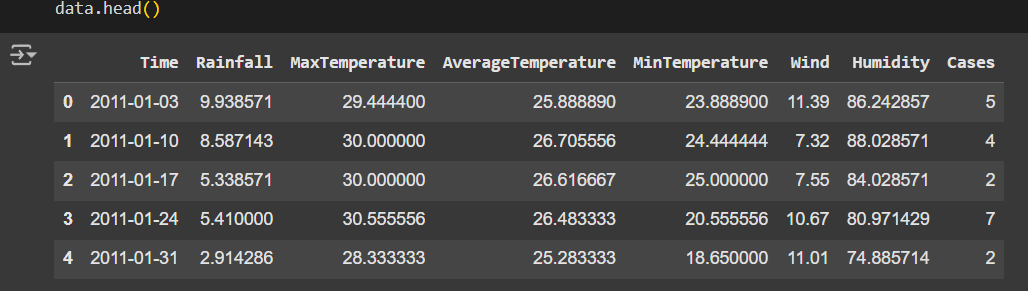
\includegraphics[width=0.95\textwidth]{data_snippet}
	\caption{Snippet of the Combined Dataset}
	\label{fig:data_snippet}
\end{figure}

\section{Exploratory Data Analysis}

\begin{figure}[h!]
	\centering
	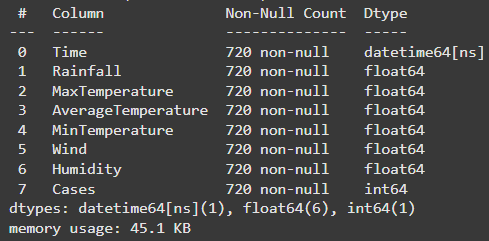
\includegraphics[width=0.75\textwidth]{data_summary}
	\caption{Data Contents}
	\label{fig:data_summary}
\end{figure}

From the summary above, the dataset consists of 720 weekly records with 8 columns:
\begin{itemize}
	\item \textbf{Time.} Weekly timestamps (e.g. "2011-w1")
	\item \textbf{Rainfall.} Weekly average rainfall (mm)
	\item \textbf{MaxTemperature, AverageTemperature, MinTemperature.} Weekly temperature data (C)
	\item \textbf{Wind.} Wind speed (m/s)
	\item \textbf{Humidity.} Weekly average humidity (\%)
	\item \textbf{Cases.} Reported dengue cases
\end{itemize}

\begin{figure}[h!]
	\centering
	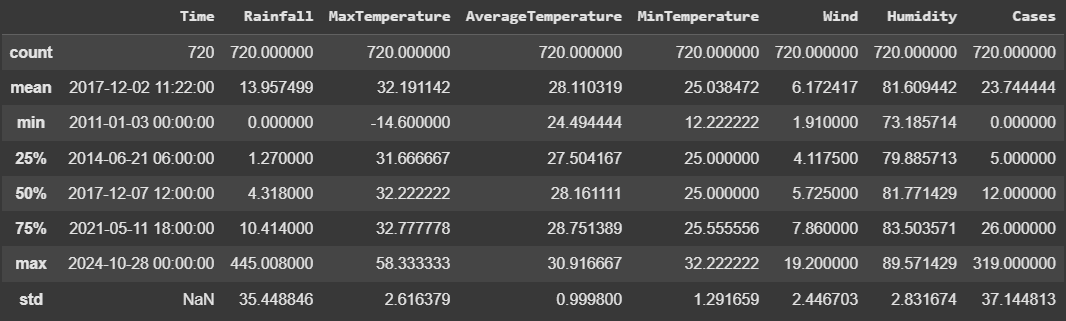
\includegraphics[width=1\textwidth]{data_stats2}
	\caption{Dataset Statistics}
	\label{fig:data_stats2}
\end{figure}

From the statistics in figure \ref{fig:data_stats2}, the number of cases ranges from 0 to 319. The average number of dengue cases per week is 23.74, with a median of 12 cases and a standard deviation of 37.14. The distribution is highly skewed, with some weeks experiencing significant number of cases (up to 319 cases). Rainfall shows a wide variation (0 to 445mm), while temperature remains relatively stable, with an average of 28.1 degree celsius. Humidity levels ranges from 73\% to 89\% with a mean of 81.6\%.

\begin{figure}[ht]
	\centering
	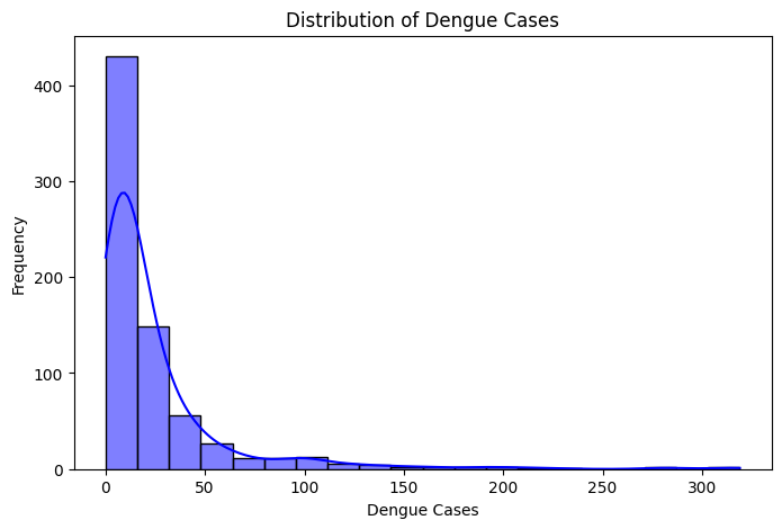
\includegraphics[width=0.75\textwidth]{data_stats}
	\caption{Distribution of Dengue Cases}
	\label{fig:data_stats}
\end{figure}

In figure \ref{fig:data_stats}, a histogram of dengue cases shows a right-skewed distribution, indicating that most weeks experience low case counts, while a few weeks record outbreaks. 
\\To further analyze the distribution, dengue cases were categorized into different intervals (Figure \ref{fig:dengue_intervals}): 0-5 cases, 6-15 cases, 16-30 cases, 31-100 cases and 101+ cases. The majority of weeks falls within the 0-5 cases and 6-15 cases categories, indicating that most weeks have low dengue cases. Meanwhile, weeks with 101+ cases are rare, suggesting that extreme outbreaks are not frequent.
\begin{figure}[ht]
	\centering
	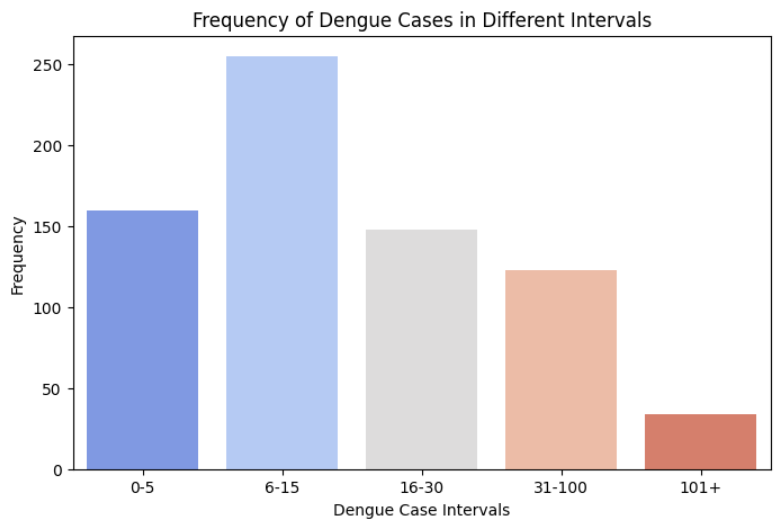
\includegraphics[width=0.75\textwidth]{dengue_intervals}
	\caption{Frequency of Dengue Cases in Different Intervals}
	\label{fig:dengue_intervals}
\end{figure}

Figure \ref{fig:data_trend} illustrates the trend of weekly dengue cases over time. The data reveals periodic spikes in the number of cases, suggesting a seasonal pattern in dengue cases. Notably, peak cases are observed during certain periods approximately 3 years, potentially aligning with specific climatic conditions such as increased rainfall or temperature changes. This underscores the importance of incorporating climate variables into the forecasting model.

\begin{figure}[ht]
	\centering
	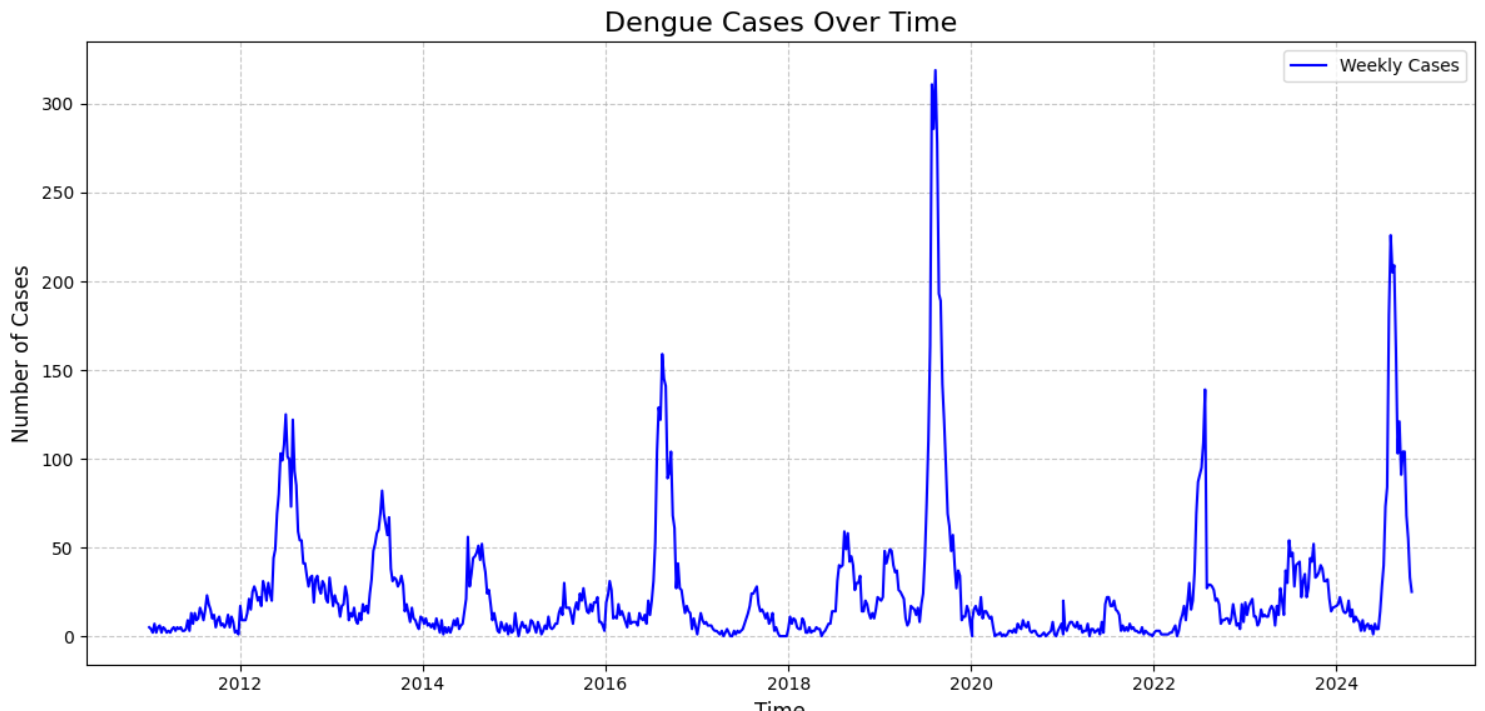
\includegraphics[width=0.90\textwidth]{dengue_trend}
	\caption{Trend of Dengue Cases}
	\label{fig:data_trend}
\end{figure}

Figure \ref{fig:correlation_bar} shows the ranking of correlation coefficients between dengue cases and selected features, including rainfall, humidity, maximum temperature, average temperature, minimum temperature, and wind speed. Among these, rainfall exhibits the highest positive correlation with dengue cases (correlation coefficient ~0.13), indicating that increased rainfall may contribute to higher cases counts. This aligns with existing studies suggesting that stagnant water from heavy rainfall creates breeding grounds for mosquitos. It is followed by humidity (~0.10), suggesting that higher humidity levels may enhance mosquito reproduction, leading to more dengue cases. Temperature has a weak to moderate positive correlation with dengue cases, with maximum temperature (0.09) showing a stronger relationship than average and minimum temperature. 

\begin{figure}[hbt!]
	\centering
	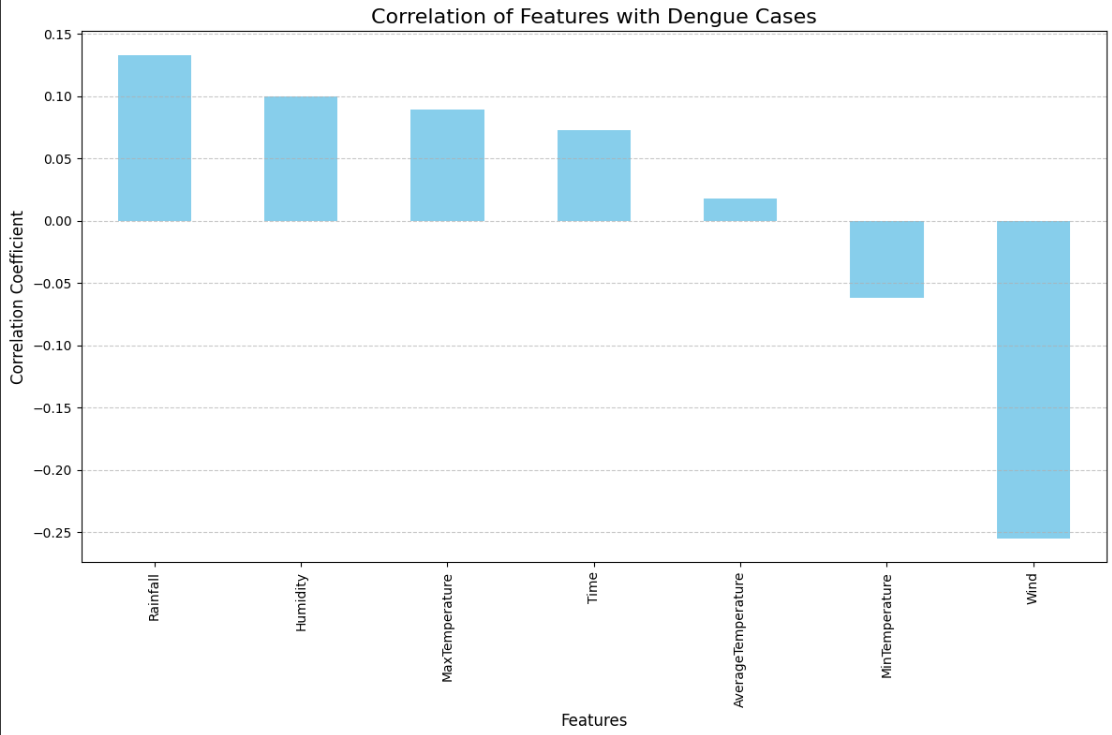
\includegraphics[width=0.75\textwidth]{correlation_bar}
	\caption{Ranking of Correlations}
	\label{fig:correlation_bar}
\end{figure}

Figure \ref{fig:lagged_correlation_bar} shows the ranking of correlation coefficients between dengue cases and selected features, with the addition of lagged effects. The analysis reveals no improvement in correlation when lagged variables are compared to direct observations. This suggests that the observed values of rainfall, humidity, and maximum temperature remain the most significant predictors for dengue case forecasting. Overall, the exploratory data analysis highlights the significance of rainfall, humidity, and max temperature variables in dengue case forecasting.

\begin{figure}[h!]
	\centering
	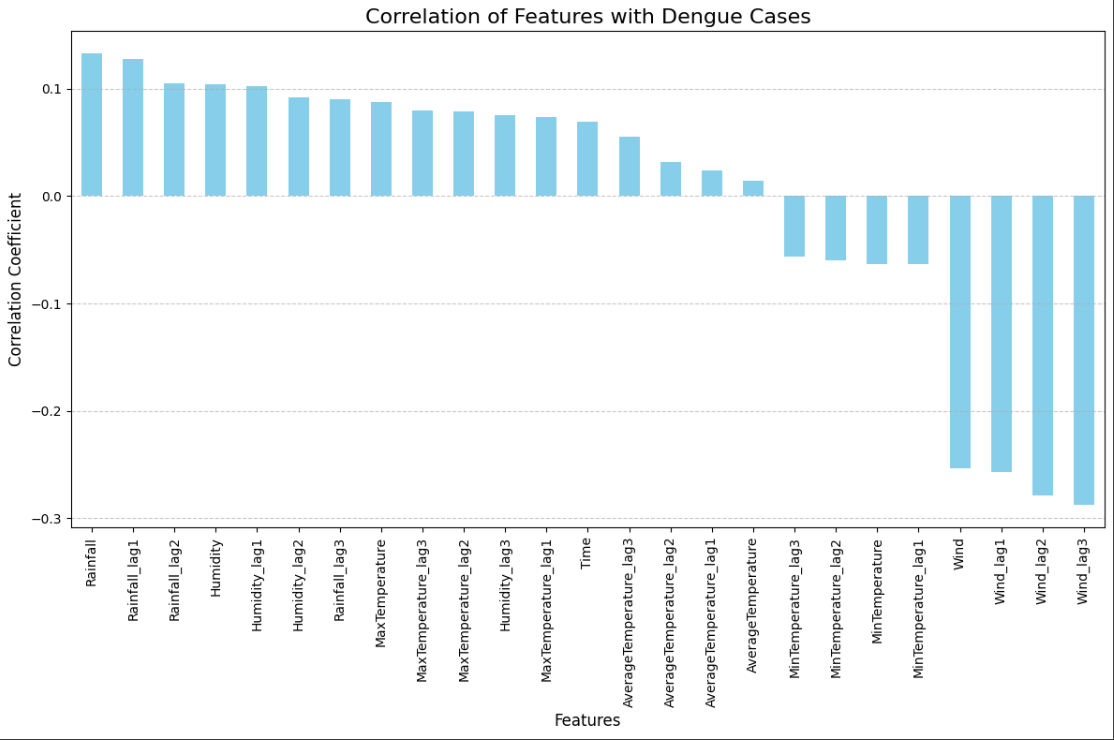
\includegraphics[width=0.75\textwidth]{lagged_correlation_bar}
	\caption{Ranking of Correlations (with lagged effects)}
	\label{fig:lagged_correlation_bar}
\end{figure}

\section{Outbreak Detection}  
To identify outbreaks, we calculated the outbreak threshold value using the historical mean as the endemic channel. The threshold is determined using the formula:  

\begin{align}  
	\text{Outbreak Threshold Value} &= \mu + 2\sigma \\  
	&= 23.744444 + 2(37.144813) \\  
	&= 23.744444 + 74.289626 \\  
	&= 98.03407  
\end{align}  

where \(\mu\) is the historical mean and \(\sigma \) is the standard deviation.

This result indicates that dengue cases exceeding 98 in Iloilo City can be considered an outbreak. However, it is important to note that this threshold serves only as a baseline. Additional parameters, such as the number of hospital beds available in the city, must be considered to compute a more effective threshold and develop an appropriate response strategy.

	
\section{Model Training Results}

The models were evaluated using three metrics: MSE, RMSE, and MAE. The table below provides a summary and comparative analysis of each model’s results across these metrics, offering insights into the strengths and limitations of each forecasting technique for dengue case prediction in Iloilo City. The lower values of the three metrics indicate better forecasting performance. Table \ref{tab:comparison_of_models} shows that the models performed differently on testing data. LSTM outperformed the other models with the lowest RMSE, MSE, and MAE while the other three models had relatively higher values for the three metrics.

\begin{table}[h!]
	\centering
	\resizebox{1\textwidth}{!}{%
		\begin{tabular}{|l|c|c|c|c|c|}
			\hline
			\textbf{Method} & \textbf{LSTM} & \textbf{Seasonal ARIMA} & \textbf{ARIMA} & \textbf{Kalman Filter} & \textbf{KF-LSTM} \\ 
			\hline
			\textbf{Testing MSE}   & 285.54 & 1261.20 & 1521.48 & 1474.82 & 785.35 \\ 
			\hline
			\textbf{Testing RMSE}  & 16.90  & 34.45  & 39.00 & 38.40 & 25.56 \\ 
			\hline
			\textbf{Testing MAE}   & 9.45  & 18.73  & 25.80 & 22.33 & 14.55 \\ 
			\hline
			\textbf{Best Parameters}   
			& \begin{tabular}[c]{@{}c@{}}Window Size: 5\\ Learning Rate: 0.01\\ Units: 64\end{tabular}  
			& (2,0,2)(0,1,1)  
			& (1,2,2) 
			& \begin{tabular}[c]{@{}c@{}}Observation Covariance: 10.0\\ Transition Covariance: 0.1 $\times$ Identity\end{tabular}
			& Same as LSTM \\ 
			\hline
		\end{tabular}%
	}
	\caption{Comparison of different models for dengue prediction}
	\label{tab:comparison_of_models}
\end{table}




\subsection{LSTM Model}
The LSTM model was tuned for the following parameters: learning rate and units. The hyperparameter tuning was conducted for each window size, finding the best parameters for each window size. Further evaluating which window size is most suitable for the prediction model, Table \ref{tab:comparison_of_lstm} shows the evaluation metrics for each window size used in the LSTM model training.
\begin{table}[h!]
	\centering
	\begin{tabular}{|l|c|c|c|c|}
		\hline
		\textbf{Window Size} & \textbf{MSE} & \textbf{RMSE} & \textbf{MAE} & \textbf{R²}\\ \hline
		\textbf{5} & \textbf{285.54} & \textbf{16.90} & \textbf{9.45} & \textbf{0.83}\\ \hline
		\textbf{10} & \textbf{334.63} & \textbf{18.29} & \textbf{9.85} & \textbf{0.80}\\ \hline
		\textbf{20} & \textbf{294.85} & \textbf{17.17} & \textbf{9.35} & \textbf{0.83}\\ \hline
	\end{tabular}
	\caption{Comparison of Window Sizes}
	\label{tab:comparison_of_lstm}
\end{table}

The results indicate that a window size of 5 weeks provides the most accurate predictions, as evidenced by the lowest MSE and RMSE values. Furthermore, the R² score of 0.83 indicates that 83\% of the variability in the target variable (cases) is explained by the independent variables (the inputs) in the model, making it a reliable configuration overall.

Figure \ref{fig:tcsv_training} illustrates the model’s performance in predicting dengue cases for each fold using a window size of 5. As shown in the plot, the training set progressively increases with each fold, mimicking a real-world scenario where more data becomes available over time for dengue prediction. Figure \ref{fig:tcsv_testing} demonstrates that the predicted cases closely follow the trend of the actual cases, indicating that the LSTM model successfully captures the underlying patterns in the data. It is also evident that as the fold number increases and the training set grows, the accuracy of the predictions on the test set improves. Despite the test data being unseen, the model exhibits a strong ability to generalize, suggesting it effectively leverages past observations to predict future trends.

\begin{figure}[H]
	\centering
	\includegraphics[width=1\textwidth]{TSCV_training}
	\caption{Training Folds - Window Size 5}
	\label{fig:tcsv_training}
\end{figure}

\begin{figure}[H]
	\centering
	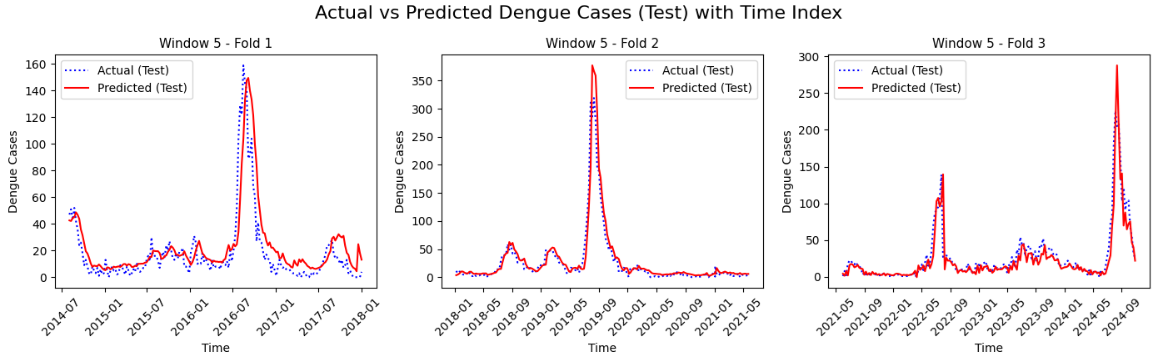
\includegraphics[width=1\textwidth]{TCSV_testing}
	\caption{Testing Folds - Window Size 5}
	\label{fig:tcsv_testing}
\end{figure}

\subsection{ARIMA Model}



\begin{figure}[H]
	\centering
	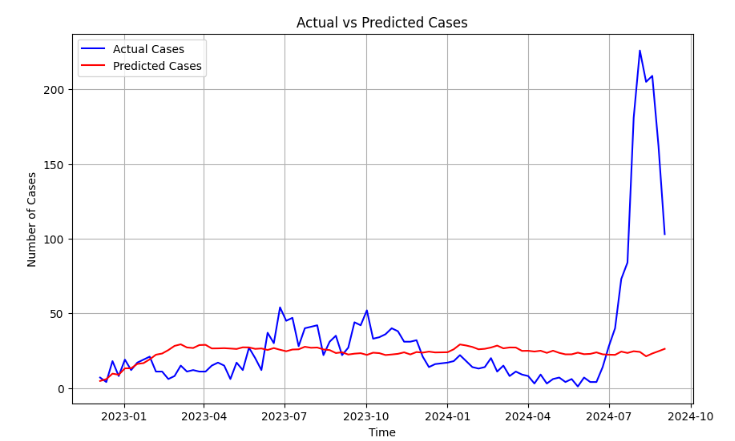
\includegraphics[width=1\textwidth]{line_graph_Arima}
	\caption{ARIMA Prediction Results for Test Set}
	\label{fig:Arima_result}
\end{figure}

The ARIMA model was developed to capture non-seasonal trends in the data. To determine the best model configuration, grid search was used to explore various combinations of ARIMA parameters, ultimately selecting \textbf{ARIMA(1, 2, 2)}. The model was iteratively refined over \textbf{400 iterations} to ensure convergence to an optimal solution. Figure \ref{fig:Arima_result} illustrates the comparison between actual and predicted dengue cases in the test set. As shown in the plot, the ARIMA model struggled to capture the non-linear characteristics and abrupt spikes in the data. Consequently, it failed to accurately reflect the fluctuations and outbreak patterns seen in the actual case counts.

The model's performance was assessed using regression metrics to evaluate its forecasting capability. The ARIMA model yielded the following error metrics:

\begin{itemize}
	\item \textbf{MSE (Mean Squared Error)}: 1521.48
	\item \textbf{RMSE (Root Mean Squared Error)}: 39.01
	\item \textbf{MAE (Mean Absolute Error)}: 25.80
\end{itemize}

\subsection{Seasonal ARIMA (SARIMA) Model}

To address the limitations of the ARIMA model, a Seasonal ARIMA (SARIMA) model was developed to capture both non-seasonal and seasonal variations in the data.

\begin{figure}[H]
	\centering
	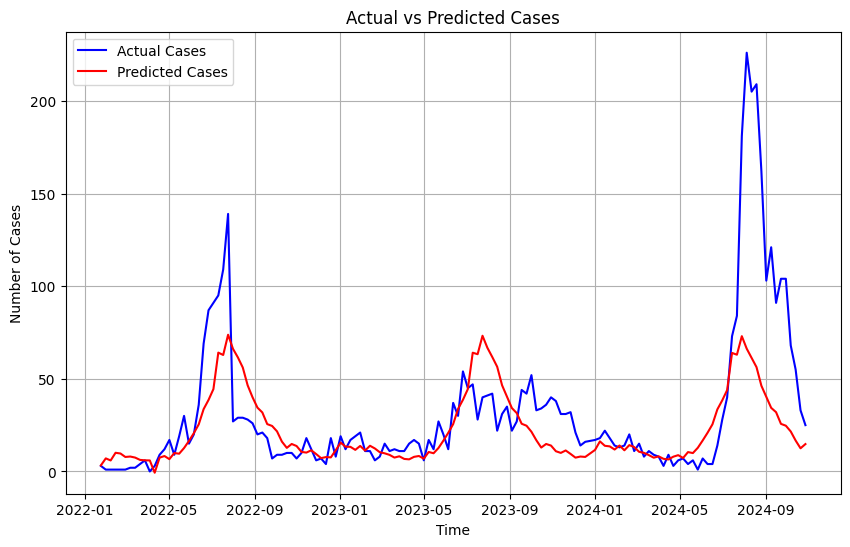
\includegraphics[width=1\textwidth]{line_graph_Sarima}
	\caption{Seasonal ARIMA Prediction Results for Test Set}
	\label{fig:Sarima_result}
\end{figure}

This model incorporates seasonal parameters, which were tuned using grid search to find the best configuration: \textbf{SARIMA(2, 0, 2)(0, 1, 1)[52]}. As with ARIMA, \textbf{400 iterations} were applied to ensure a robust fit. As shown in Figure \ref{fig:Sarima_result}, the SARIMA model demonstrates a notable improvement in performance. Unlike its non-seasonal counterpart, it effectively captures the general trend and aligns more closely with the peaks observed in the actual dengue cases, indicating its ability to model seasonal dynamics.

The model's performance was assessed using regression metrics to evaluate its forecasting capability. The SARIMA model yielded the following error metrics: \begin{itemize} \item \textbf{MSE}: 1109.69 \item \textbf{RMSE}: 33.31 \item \textbf{MAE}: 18.09 \end{itemize} The lower error values, when compared to the ARIMA model, highlight the SARIMA model's superior capability in forecasting dengue cases. Its effectiveness in capturing seasonal patterns contributed to a more accurate representation of the actual cases.

After training the model, the SARIMA model was validated using the same Time Series Cross-Validation strategy employed in the LSTM model. Table \ref{tab:tcsv_sarima} presents the performance metrics for each fold, as well as the average metrics across all folds. The average RMSE and MAE values were close to those obtained during the initial training phase, indicating that the SARIMA model performed consistently across different time segments.

\begin{table}[h!]
	\centering
	\begin{tabular}{|l|c|c|c|}
		\hline
		\textbf{Fold} & \textbf{MSE} & \textbf{RMSE} & \textbf{MAE} \\
		\hline
		1 & 659.68  & 25.68 & 16.00 \\
		2 & 2127.49 & 46.12 & 21.30 \\
		3 & 996.43  & 31.56 & 18.89 \\
		\hline
		\textbf{Average} & \textbf{1261.20} & \textbf{34.45} & \textbf{18.73} \\
		\hline
	\end{tabular}
	\caption{Comparison of SARIMA performance for each fold}
	\label{tab:tcsv_sarima}
\end{table}


\subsection{Kalman Filter Model}

Figure \ref{fig:Kalman_result} shows the comparison between the actual dengue cases and the predicted values on the test set. As illustrated in the plot, the Kalman Filter model demonstrates a moderate ability to follow the general trend of the actual data. While it effectively captures some rising and falling patterns, it still struggles to accurately replicate the sharp peaks and extreme values found in the real case counts. This limitation is particularly noticeable during the large spikes in 2022 and 2024. The model’s performance was evaluated using standard regression metrics. The results are as follows:
\[
\text{MSE} = 1474.82, \quad
\text{RMSE} = 38.40, \quad
\text{MAE} = 22.34
\]
\begin{figure}[H]
	\centering
	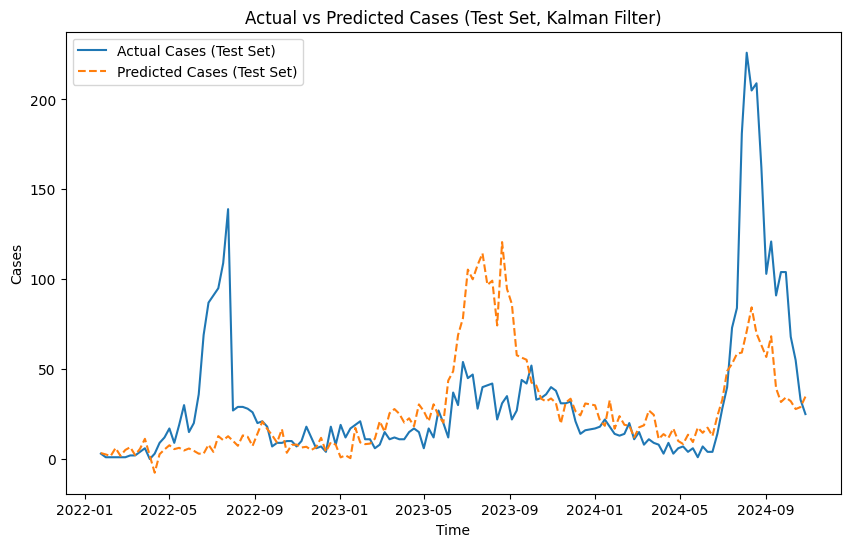
\includegraphics[width=1\textwidth]{line_graph_Kalman}
	\caption{Kalman Filter Prediction Results for Test Set}
	\label{fig:Kalman_result}
\end{figure}

The Kalman Filter was then combined with the LSTM model in order to see improvements in its predictions. Table \ref{tab:tcsv_kflstm} shows the metrics across three folds using the same Time Series Cross Validation Strategy employed in the previous models to see how it performed on different time segments.

\begin{table}[h!]
	\centering
	\begin{tabular}{|l|c|c|c|}
		\hline
		\textbf{Fold} & \textbf{MSE} & \textbf{RMSE} & \textbf{MAE} \\
		\hline
		1 & 113.59  & 10.66 & 6.42 \\
		2 & 752.51 & 27.43 & 12.11 \\
		3 & 1489.95  & 38.60 & 25.13 \\
		\hline
		\textbf{Average} & \textbf{785.35} & \textbf{25.56} & \textbf{14.55} \\
		\hline
	\end{tabular}
	\caption{Comparison of KF-LSTM performance for each fold}
	\label{tab:tcsv_kflstm}
\end{table}

As can be seen in the table above, the performance of the hybrid model demonstrated improvements in all metrics as compared to just using the Kalman Filter alone.

\section{Model Simulation}
To evaluate the LSTM model's real-world forecasting ability, a simulation was conducted to predict dengue cases for the year 2025. The model was trained exclusively on data from 2011 to 2024, using both dengue cases and weather variables. Importantly, the actual dengue case values for 2025 were never included during training. Instead, only the weather variables collected for 2025 were input into the model to generate predictions for that year. After prediction, the forecasted dengue cases for 2025 were compared against the true observed cases to assess the model’s accuracy. Figure \ref{fig:modeltesting} shows that the predicted values closely follow the trend, although it may overestimate the dengue cases in some weeks. 

\begin{figure}[H]
	\centering
	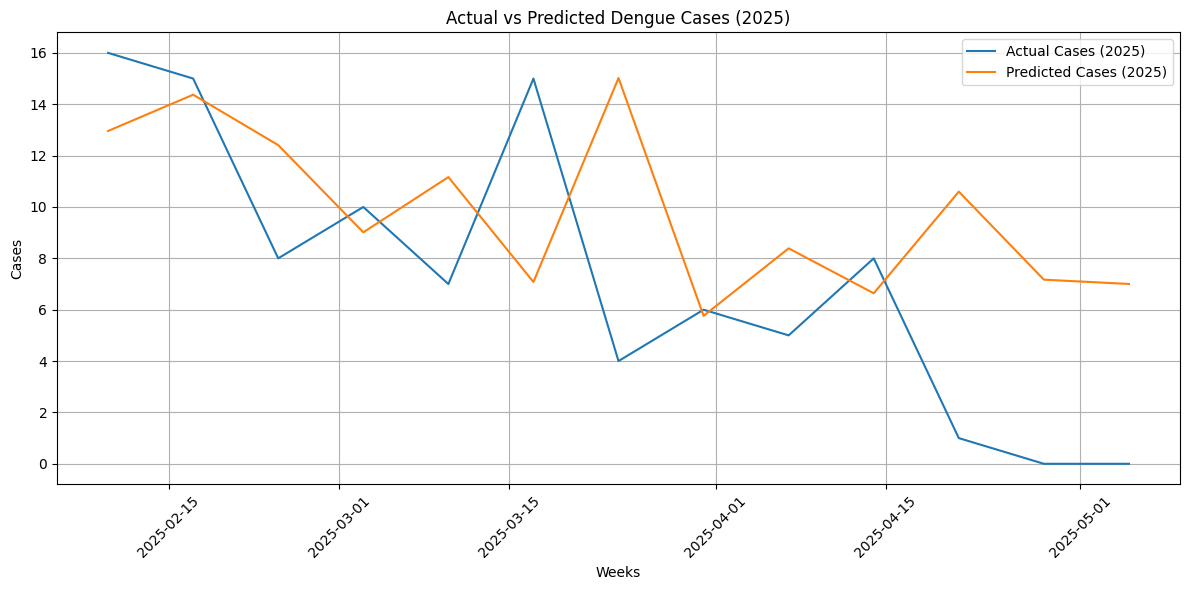
\includegraphics[width=1\textwidth]{modeltesting}
	\caption{Predicted vs Actual Dengue Cases 2025}
	\label{fig:modeltesting}
\end{figure}

\section{System Prototype}
\subsection{Home Page}
The Home Page is intended for all visitors of the web application. The Analytics Dashboard, which displays relevant statistics for dengue cases at a certain year and location, is the primary component highlighted, as seen in Figure \ref{fig:home_page}. This component includes a combo chart that graphs the number of dengue cases and deaths per week in a specific year, a choropleth map that tracks the number of dengue cases per location, and various bar charts that indicate the top locations affected by dengue. 
\begin{figure}[H]
	\centering
	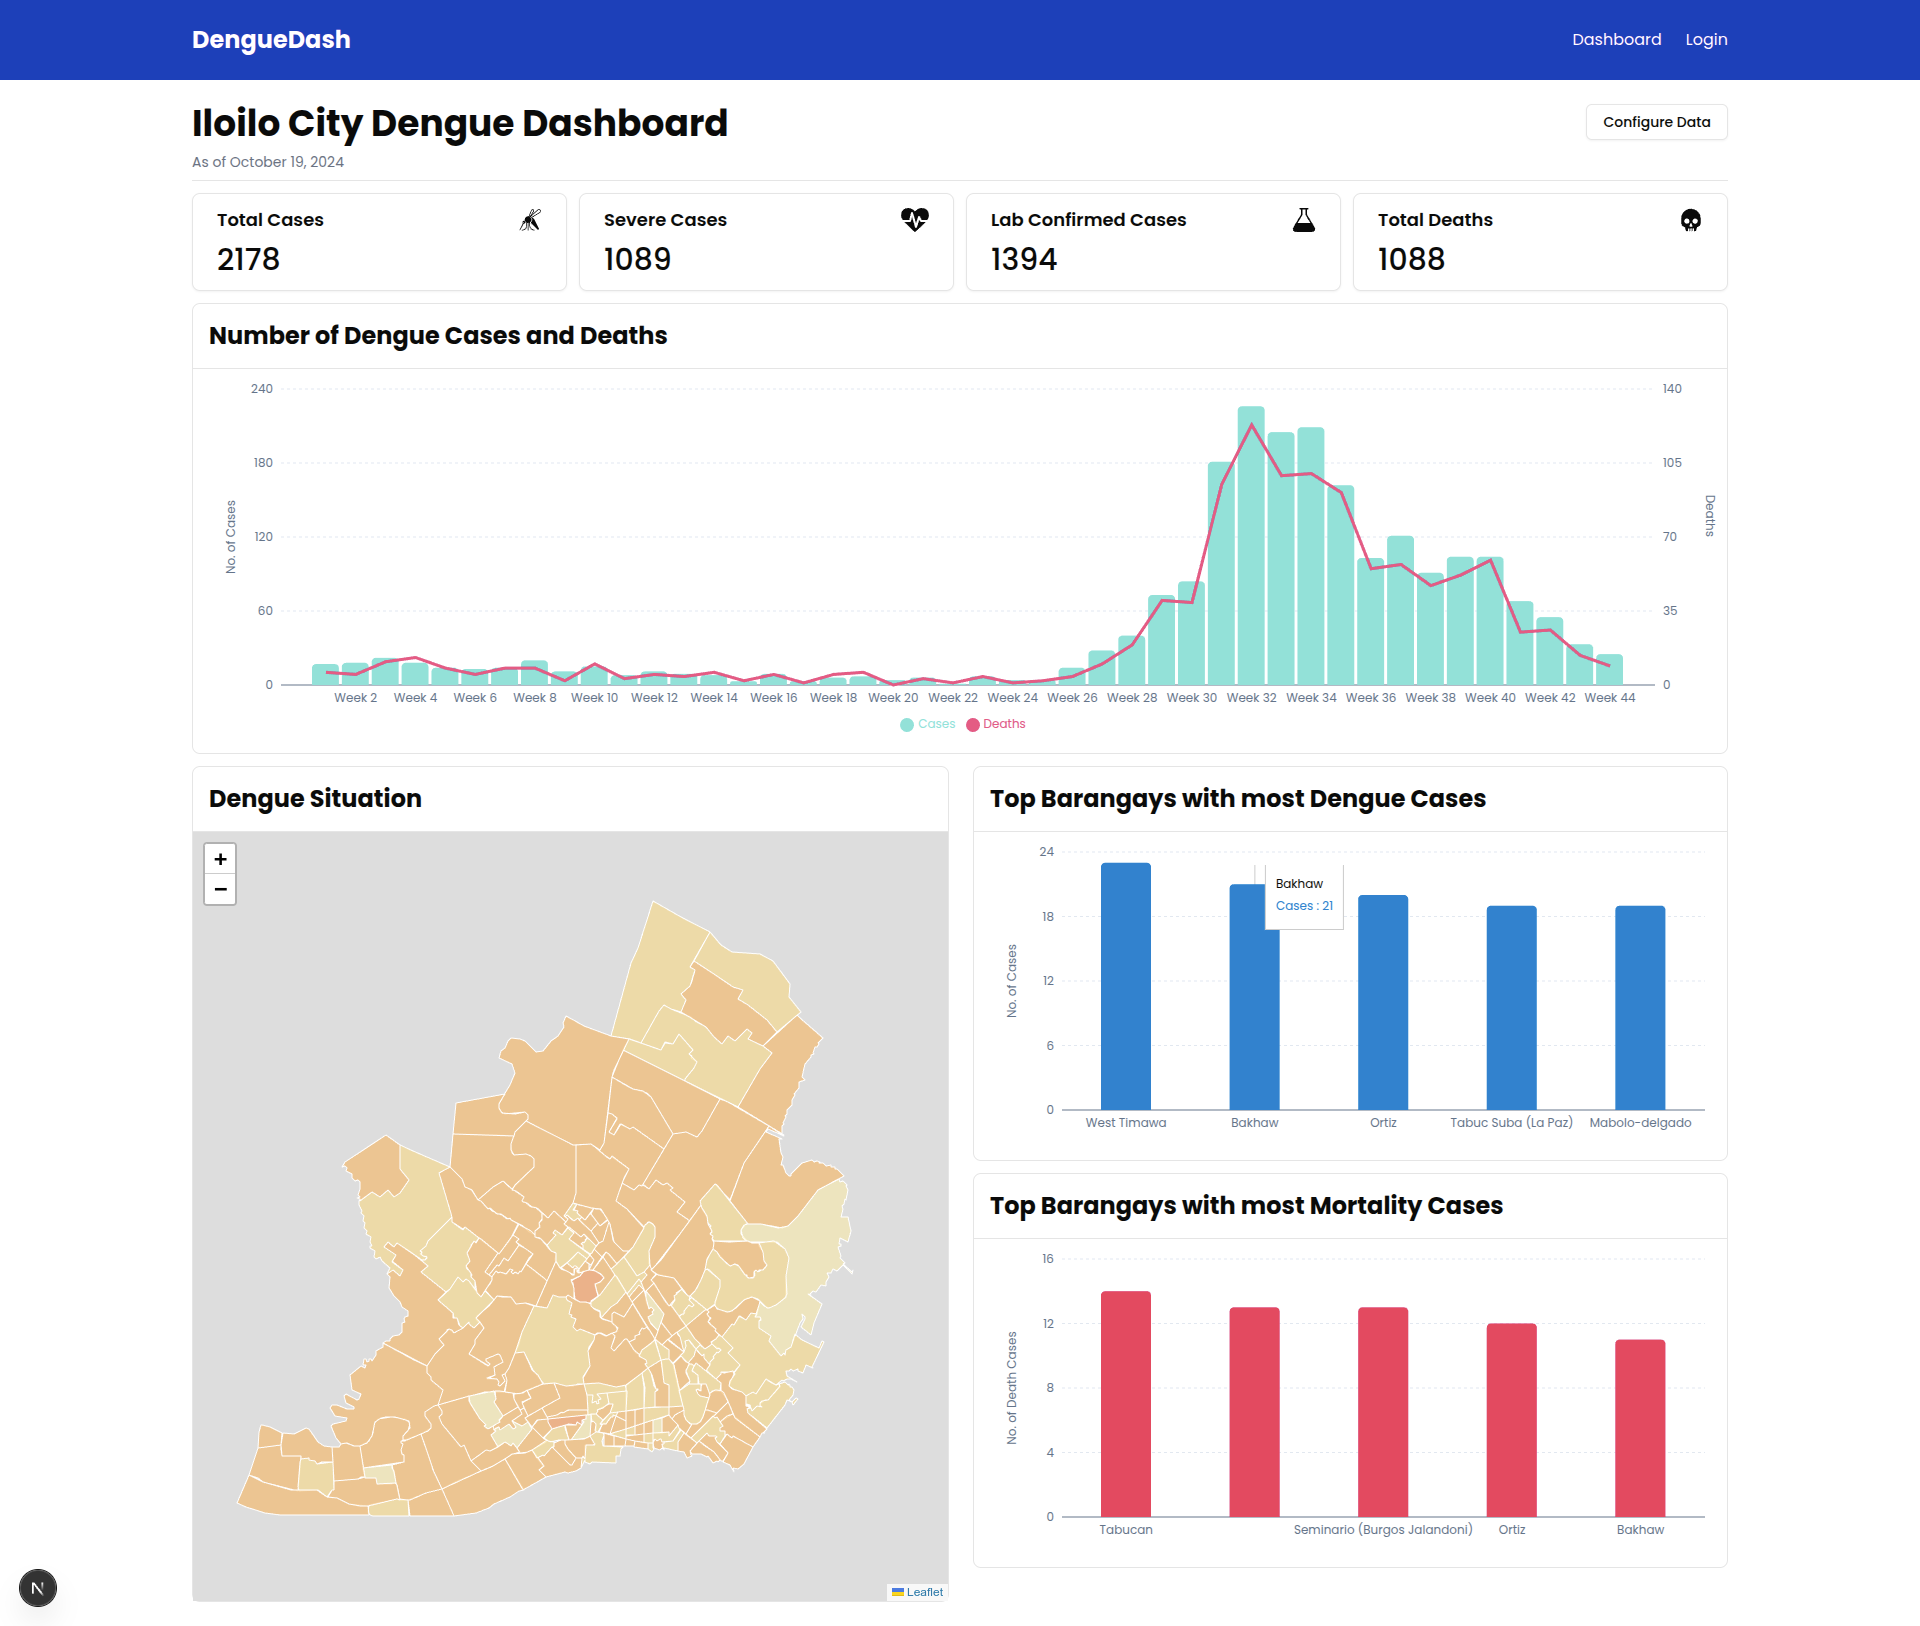
\includegraphics[width=1\textwidth]{home_page}
	\caption{Home Page}
	\label{fig:home_page}
\end{figure}

\subsection{User Registration, Login, and Authentication}
The registration page, as shown in Figure \ref{fig:registration_page}, serves as a gateway to access the authenticated pages of the web application. Only prospected encoders can create an account since administrator accounts are only made by existing administrator accounts to protect the data's integrity in production. After registering, the "encoder account" cannot access the authorized pages yet as it needs to be verified first by an administrator managing the unit the user entered. Once verified, the user can log in to the system through the page shown in Figure \ref{fig:login_page}. After entering the correct credentials, which consist of an email and password, the system uses HTTP-only cookies containing JSON Web Tokens (JWT) to prevent vulnerability to Cross-site Scripting (XSS) attacks. It will then proceed to the appropriate page the type of user belongs to. 
\begin{figure}[H]
	\centering
	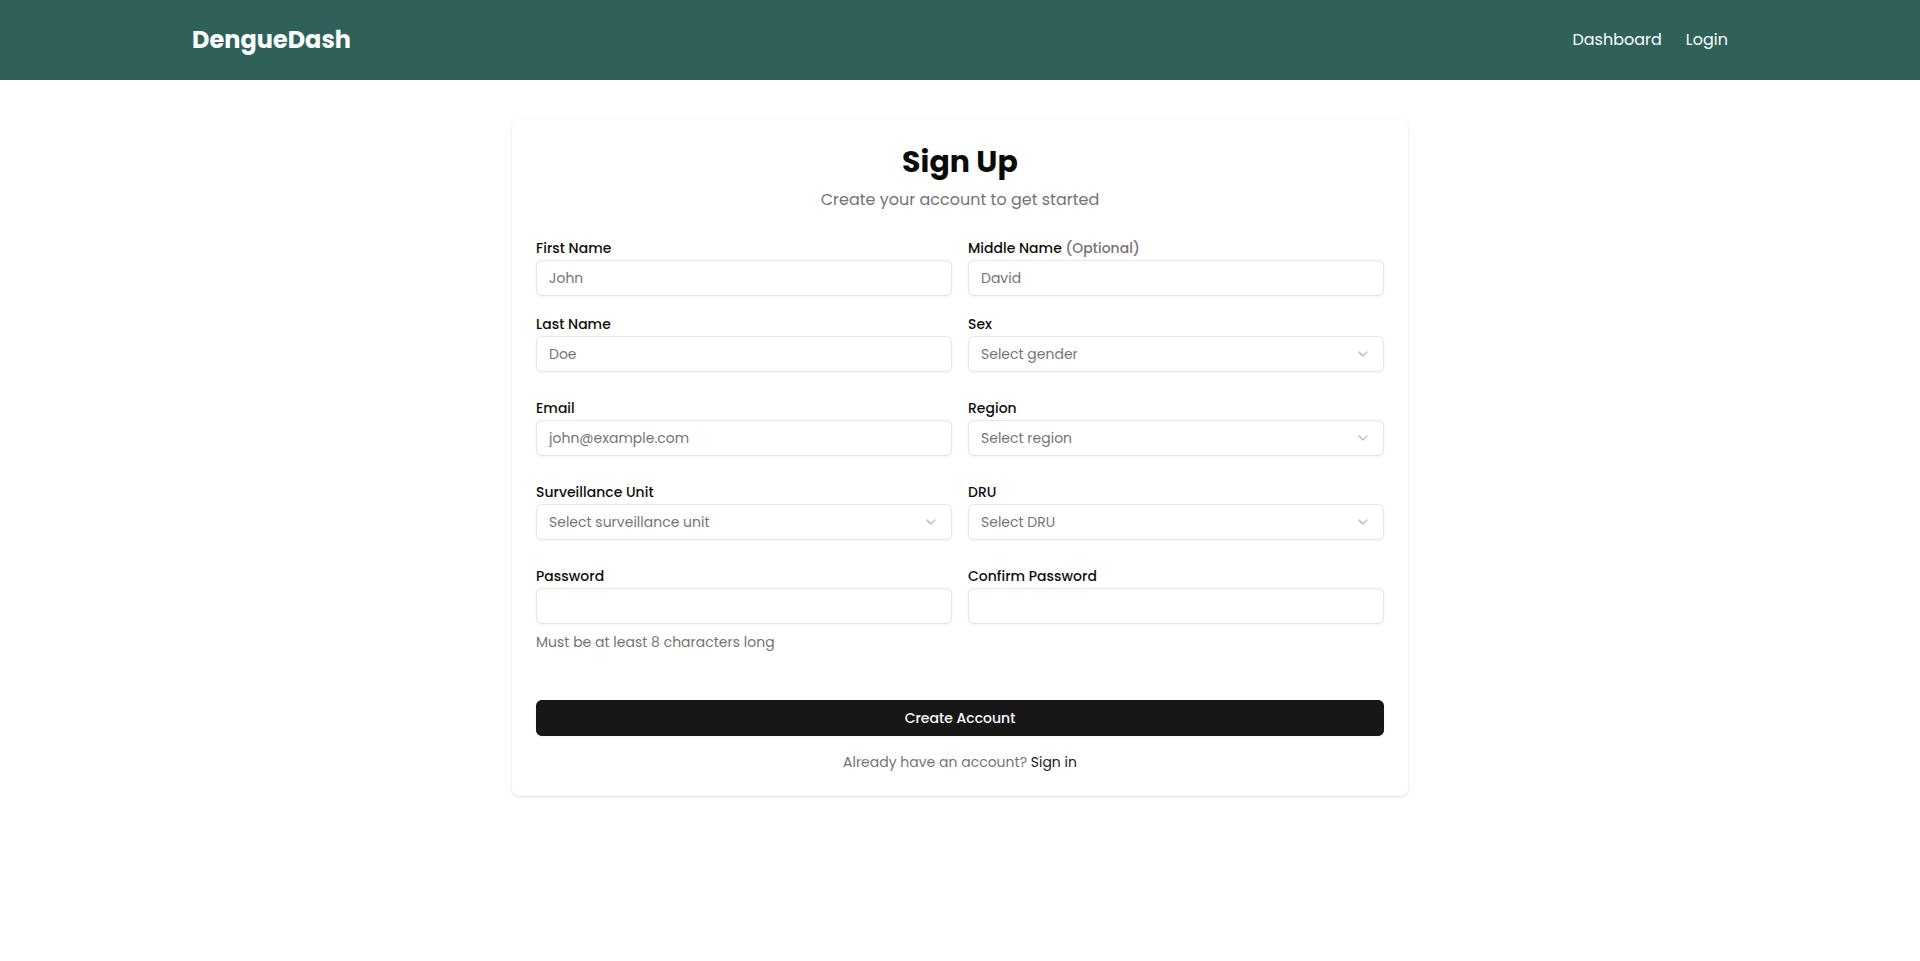
\includegraphics[width=1\textwidth]{registration_page}
	\caption{Sign Up Page}
	\label{fig:registration_page}
\end{figure}

\begin{figure}[H]
	\centering
	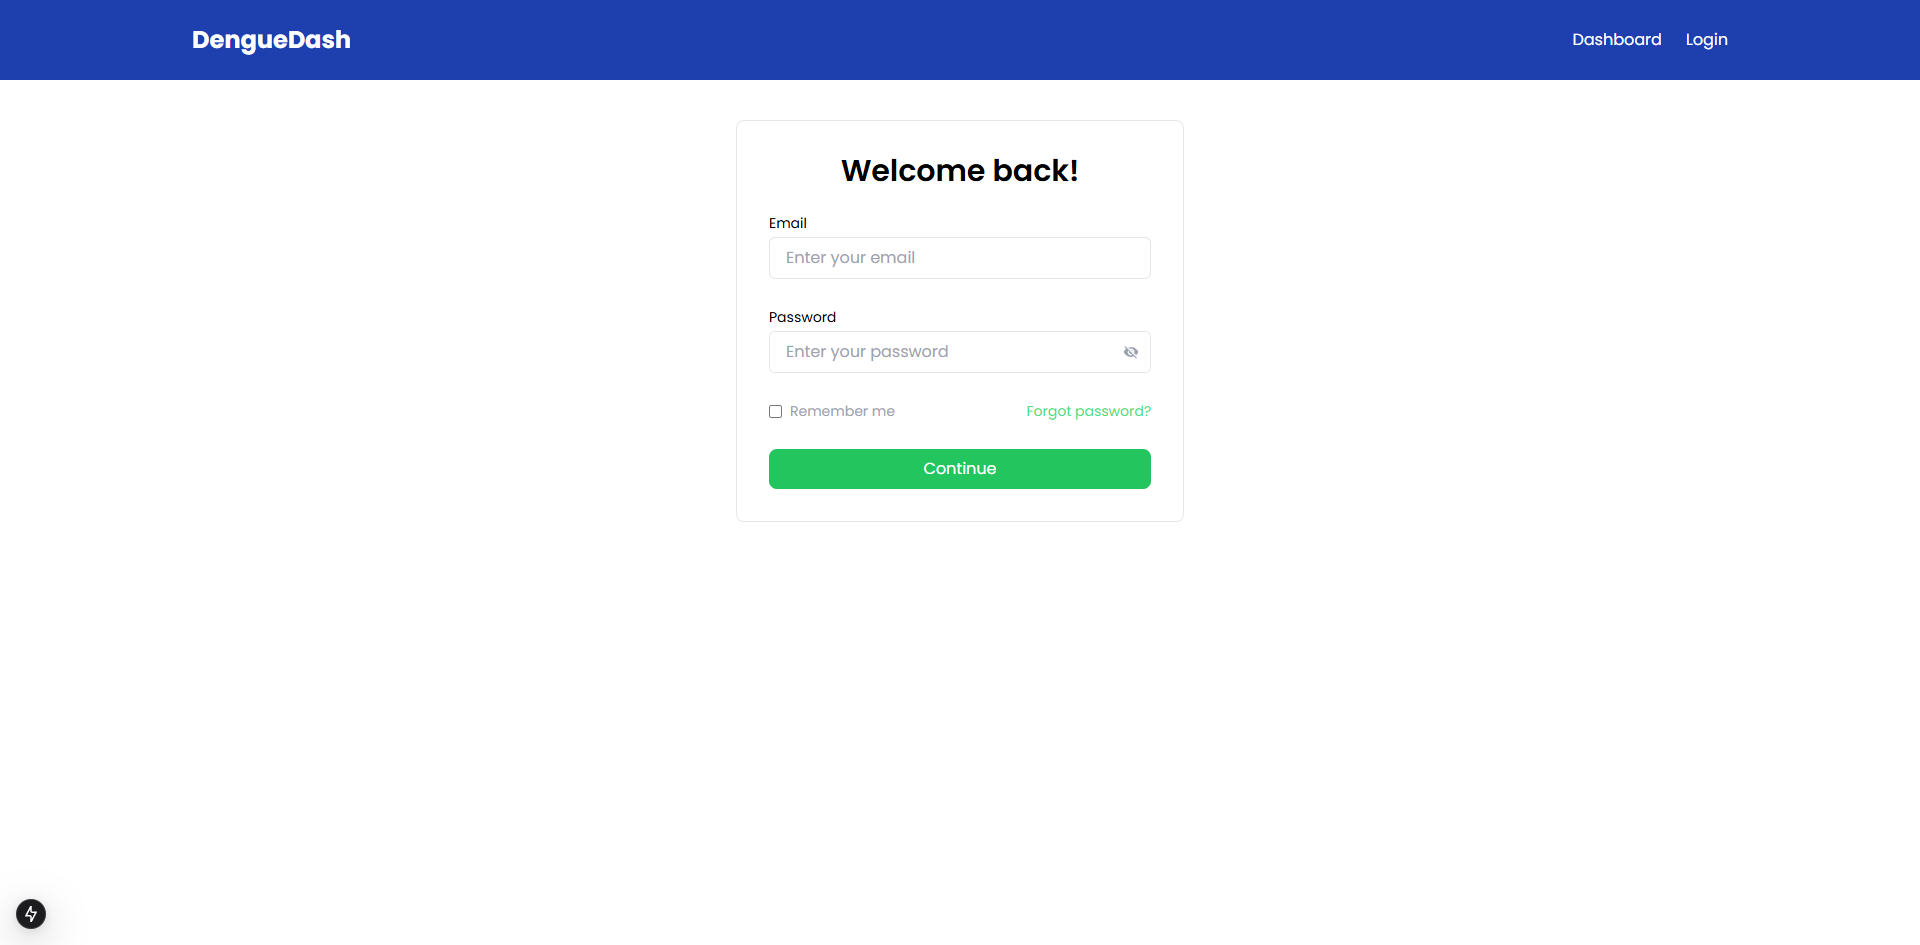
\includegraphics[width=1\textwidth]{login_page}
	\caption{Login Page}
	\label{fig:login_page}
\end{figure}

\subsection{Encoder Interface}
\subsubsection{Case Report Form}
Figures \ref{fig:case_report_form_1} and \ref{fig:case_report_form_2} show the digitized counterpart of the form obtained from the Iloilo Provincial Epidemiology and Surveillance Unit. As the system aims to support expandability for future features, some fields were modified to accommodate more detailed input. It is worth noting that all of the included fields adhere to the latest Philippine Integrated Disease and Surveillance Response (PIDSR) Dengue Forms, which the referenced form was based on. By doing this, if implemented on a national scale, the transition between targeted users will be easier. Moreover, the case form includes the patient's basic information, dengue vaccination status, consultation details, laboratory results, and the outcome. On the other hand, encoders can also create case records using a "bulk upload" feature that makes use of a formatted CSV file template. As shown in Figure \ref{fig:bulk_upload}, an encoder can download the template using the "Download Template" button, and insert multiple records inside the file, then upload it by clicking the "Click to upload" button. The web application automatically checks the file for data inconsistencies and validation. 
\begin{figure}[H]
	\centering
	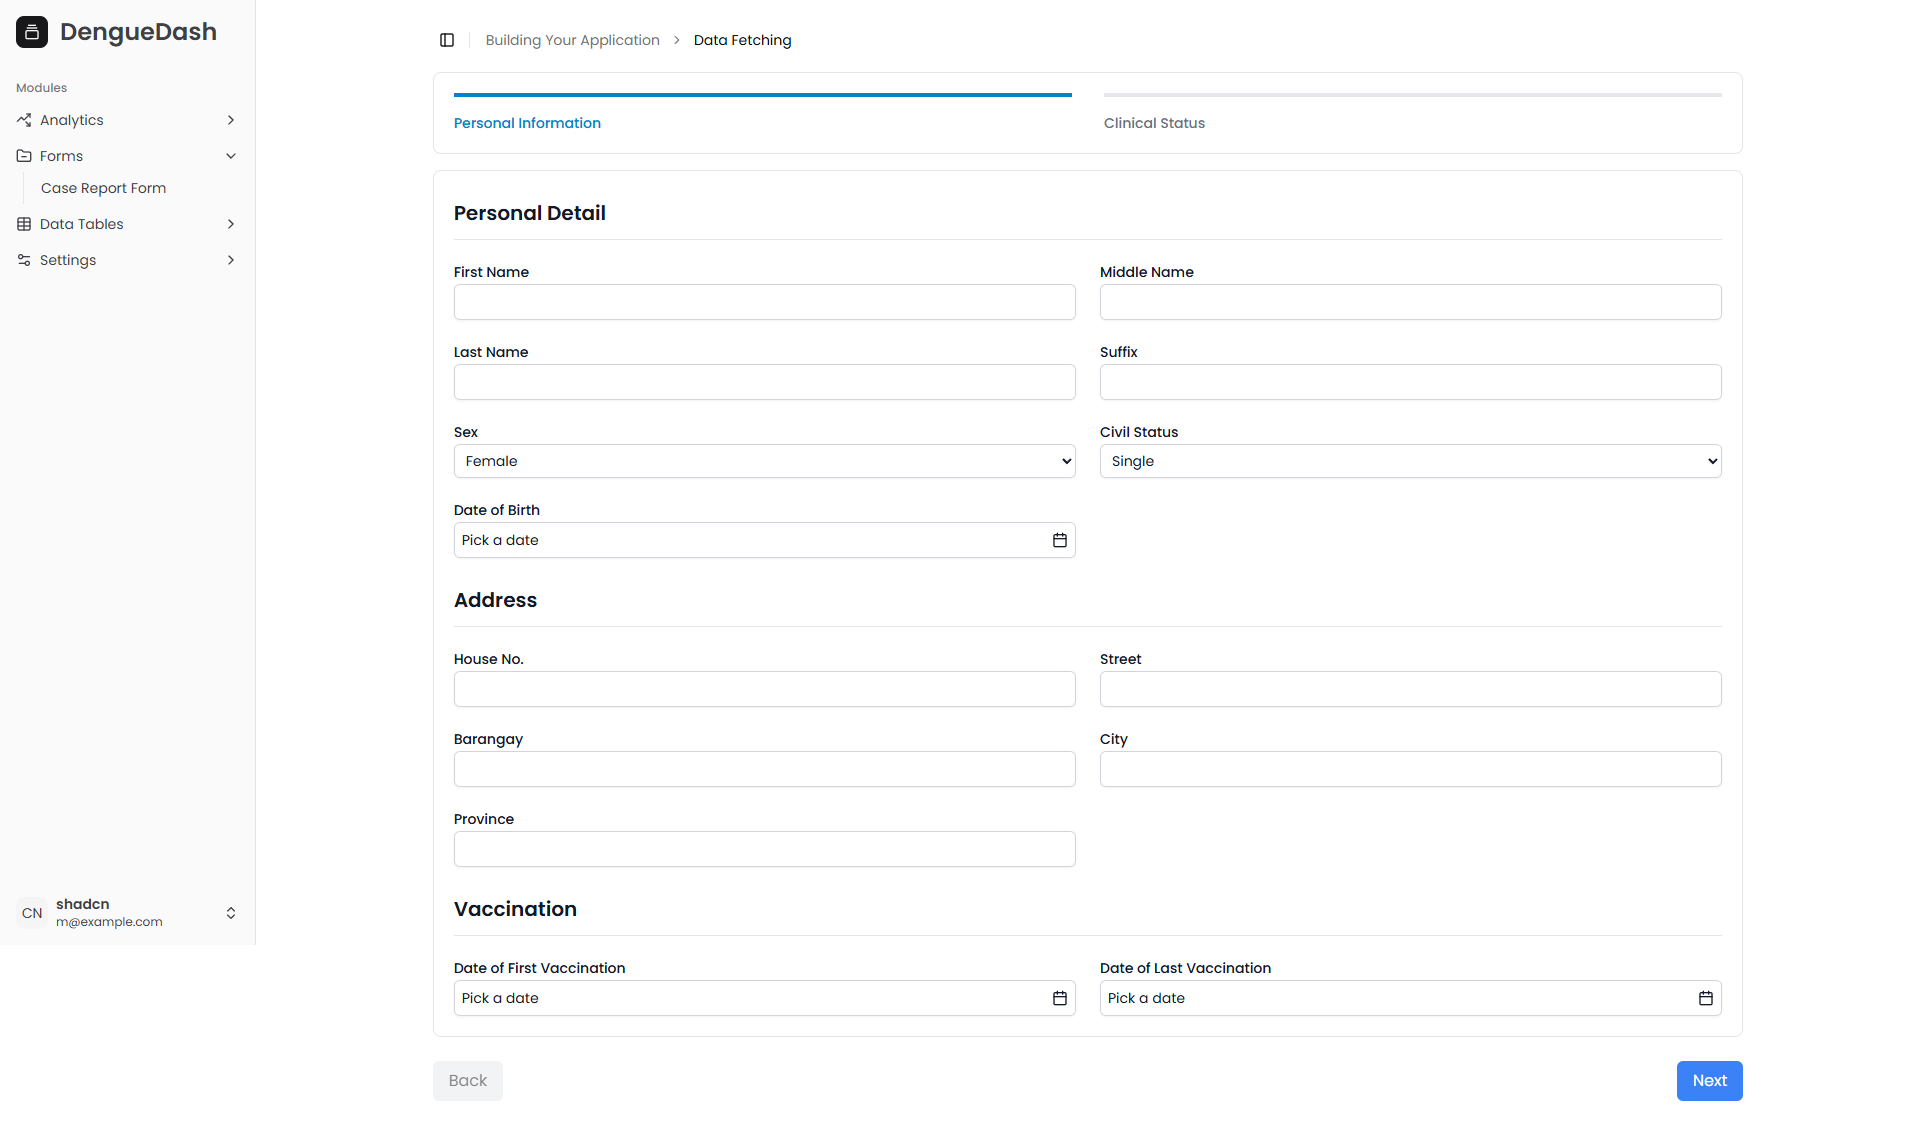
\includegraphics[width=1\textwidth]{case_report_form_1}
	\caption{First Part of Case Report Form}
	\label{fig:case_report_form_1}
\end{figure}
\begin{figure}[H]
	\centering
	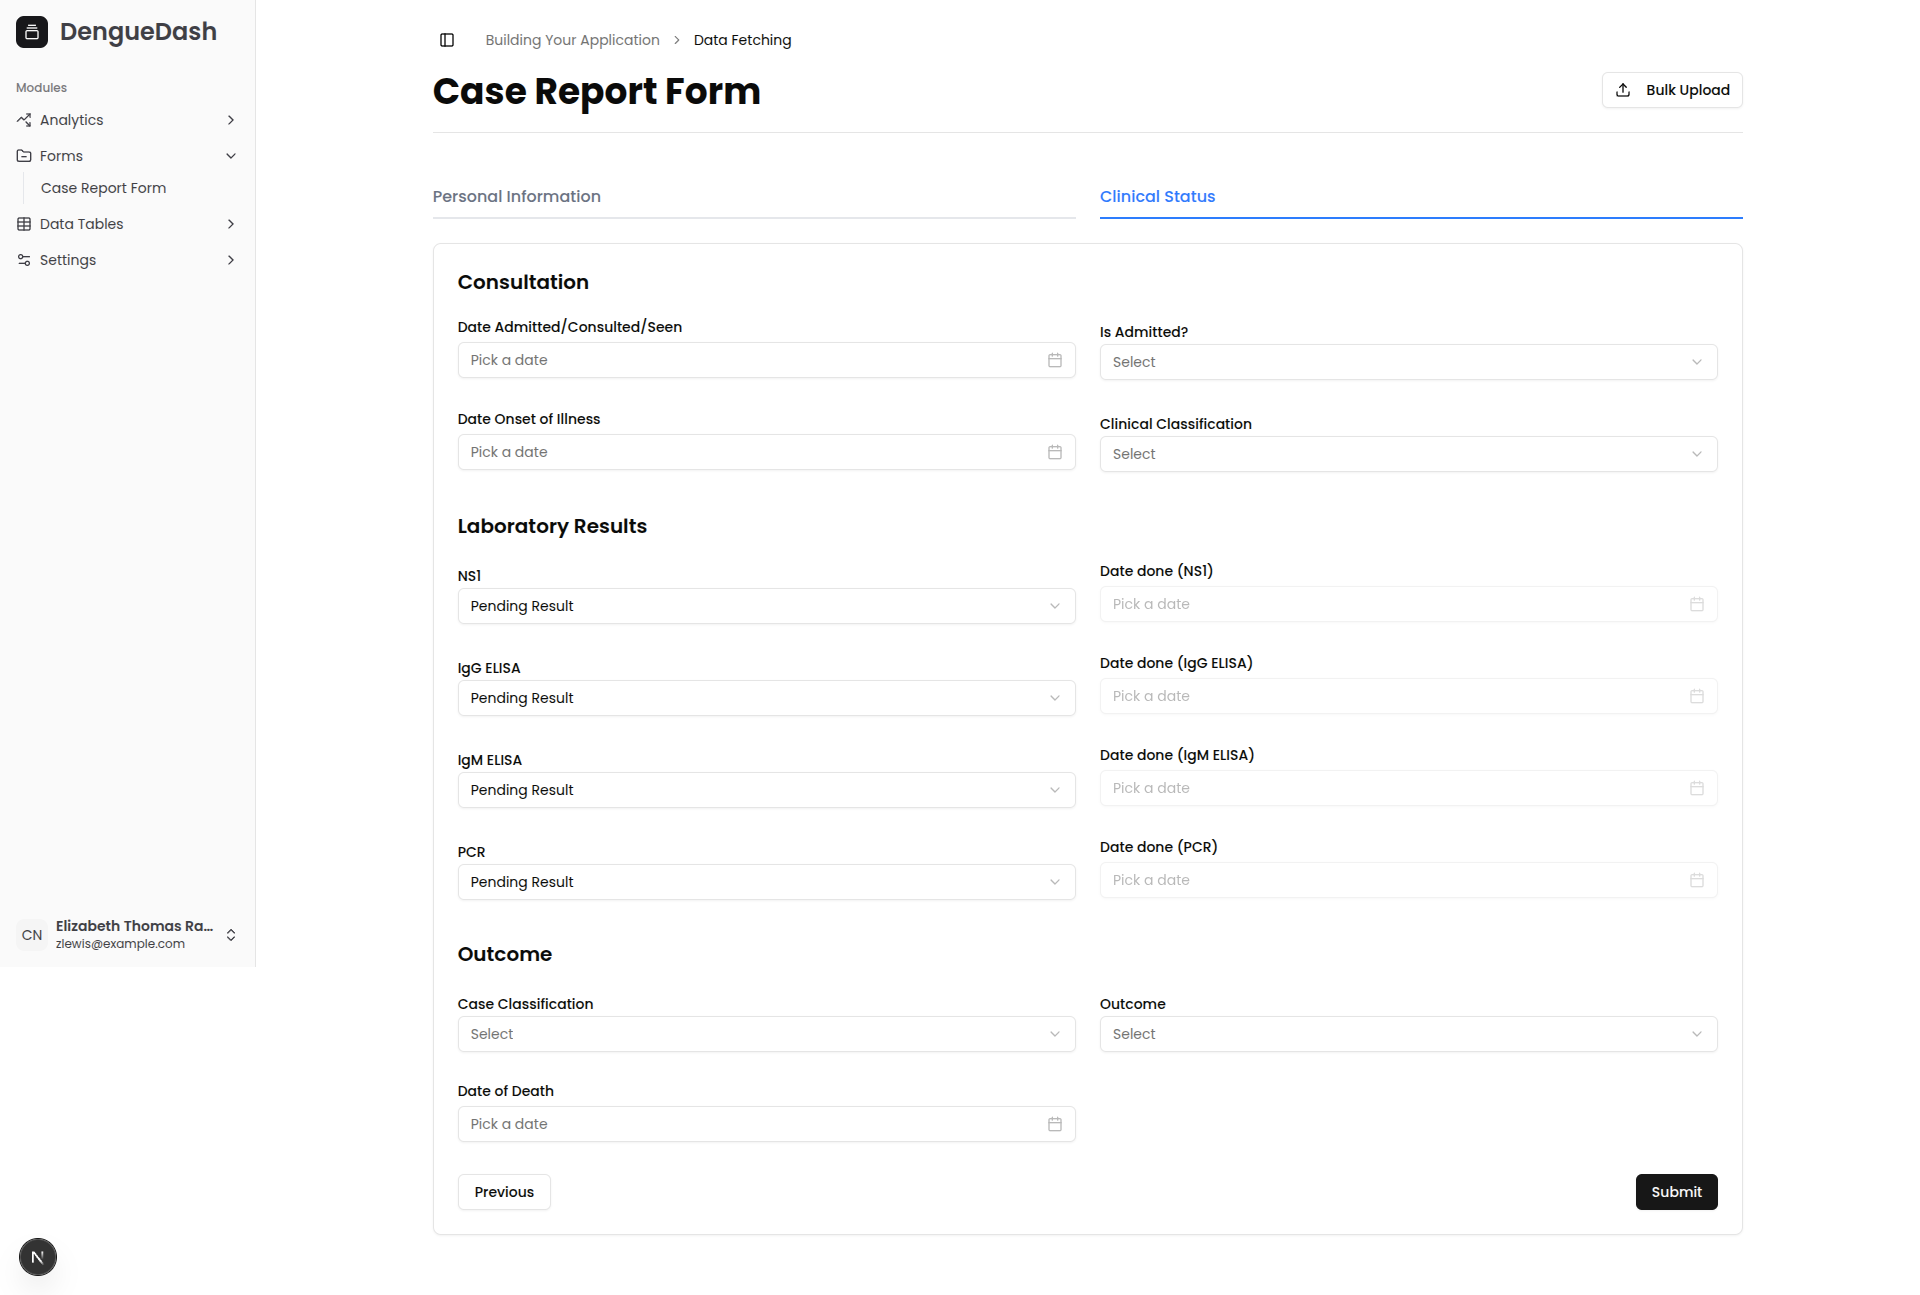
\includegraphics[width=1\textwidth]{case_report_form_2}
	\caption{Second Part of Case Report Form}
	\label{fig:case_report_form_2}
\end{figure}
\begin{figure}[H]
	\centering
	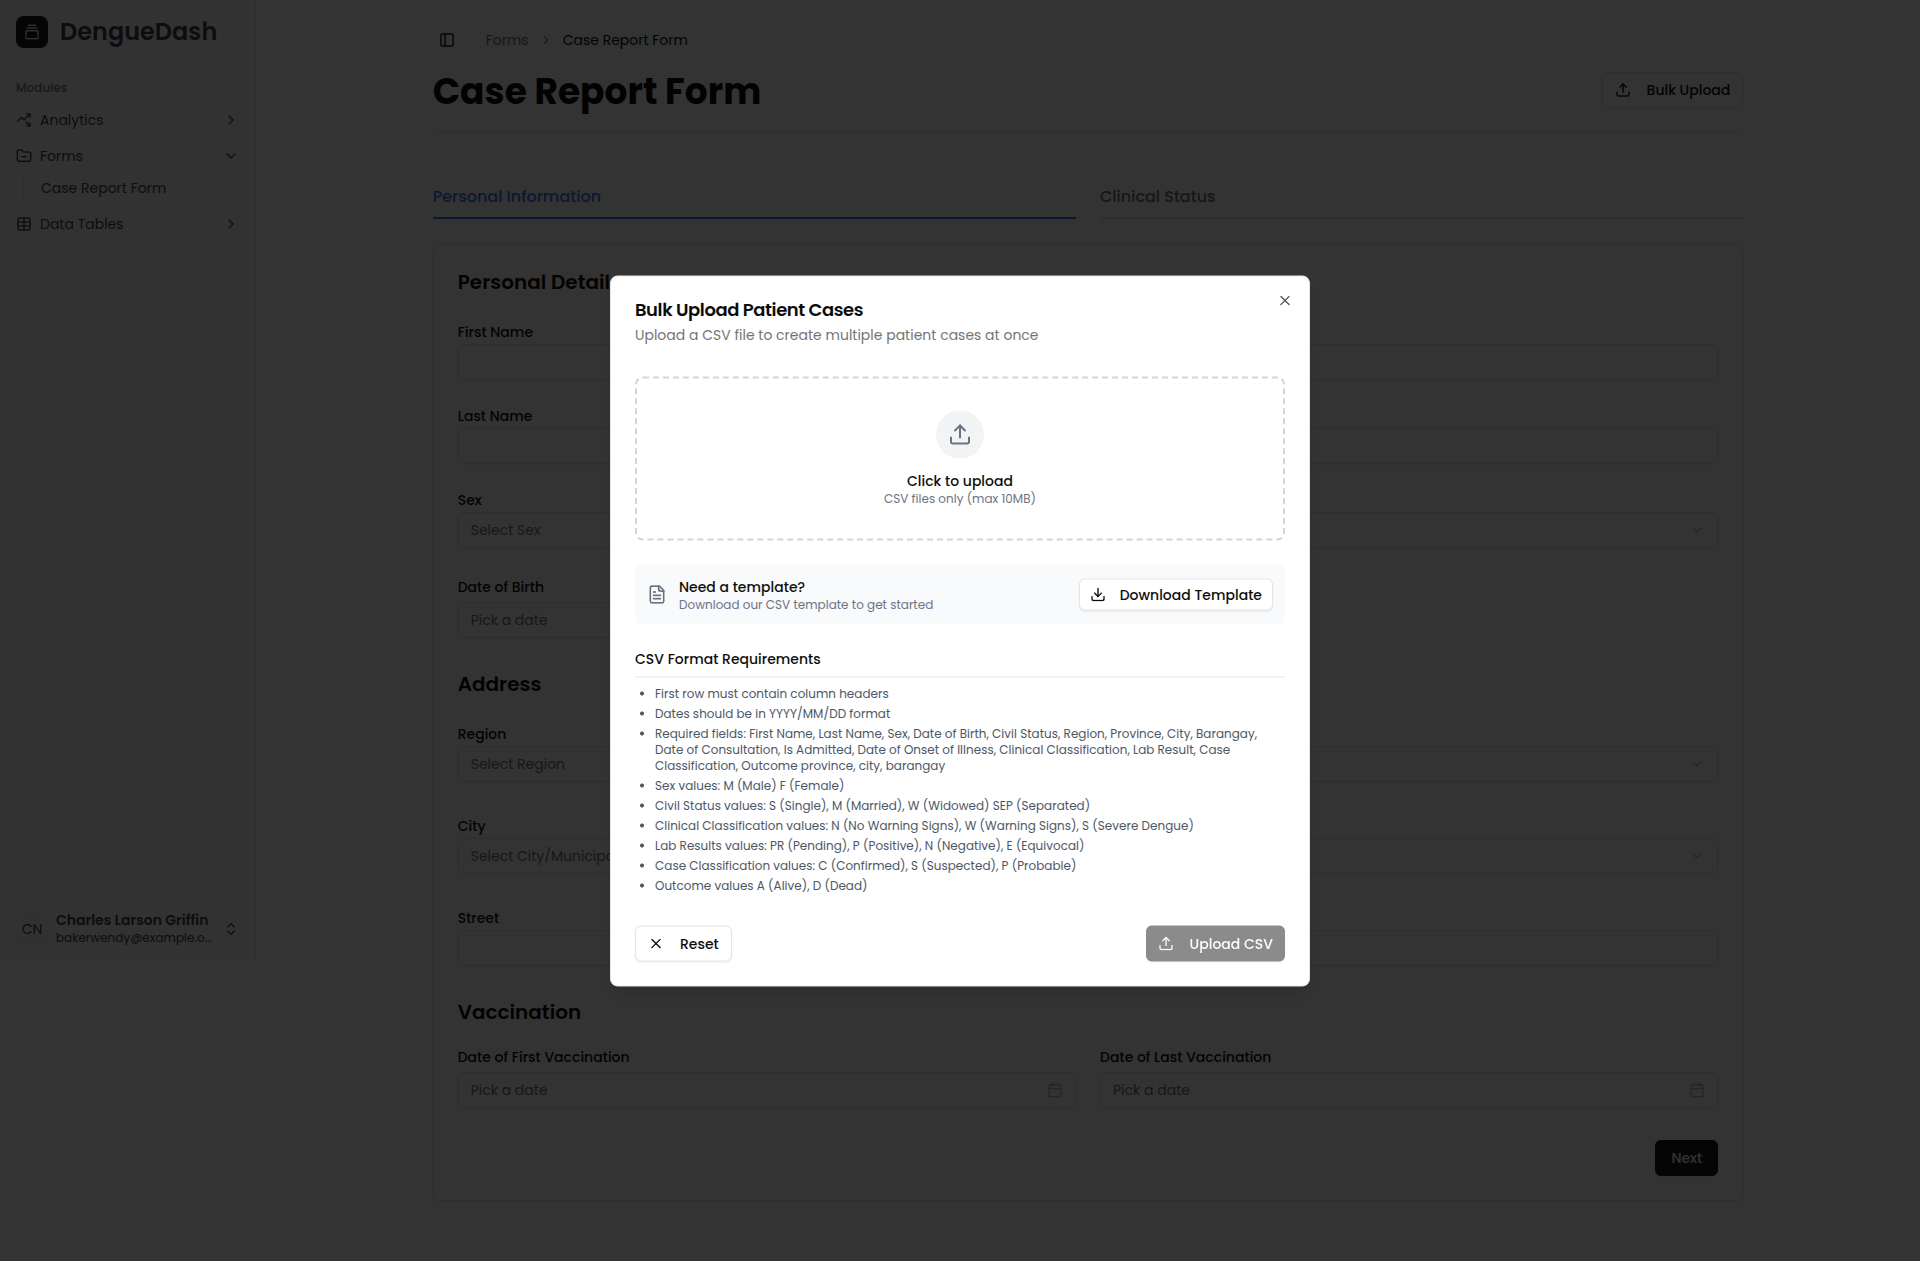
\includegraphics[width=1\textwidth]{bulk_upload}
	\caption{Bulk Upload of Cases using CSV}
	\label{fig:bulk_upload}
\end{figure}

\subsubsection{Browsing, Update, and Deletion of Records}
Once the data generated from the case report form or the bulk upload is validated, it will be assigned as a new case and can be accessed through the Dengue Reports page, as shown in Figure \ref{fig:dengue_reports}. The said page displays basic information about the patient related to a specific case, including their name, address, date of consultation, and clinical and case classifications. It is also worth noting that it only shows cases the user is permitted to view. For example, in a local Disease Reporting Unit (DRU) setting, the user can only access records that belong to the same DRU. On the other hand, in a consolidated surveillance unit such as a regional, provincial, or city quarter, its users can view all the records from all the DRUs that report to them. Moving forward, Figure \ref{fig:detailed_case_report} shows the detailed case report of the patient on a particular consultation date. 
\begin{figure}[H]
	\centering
	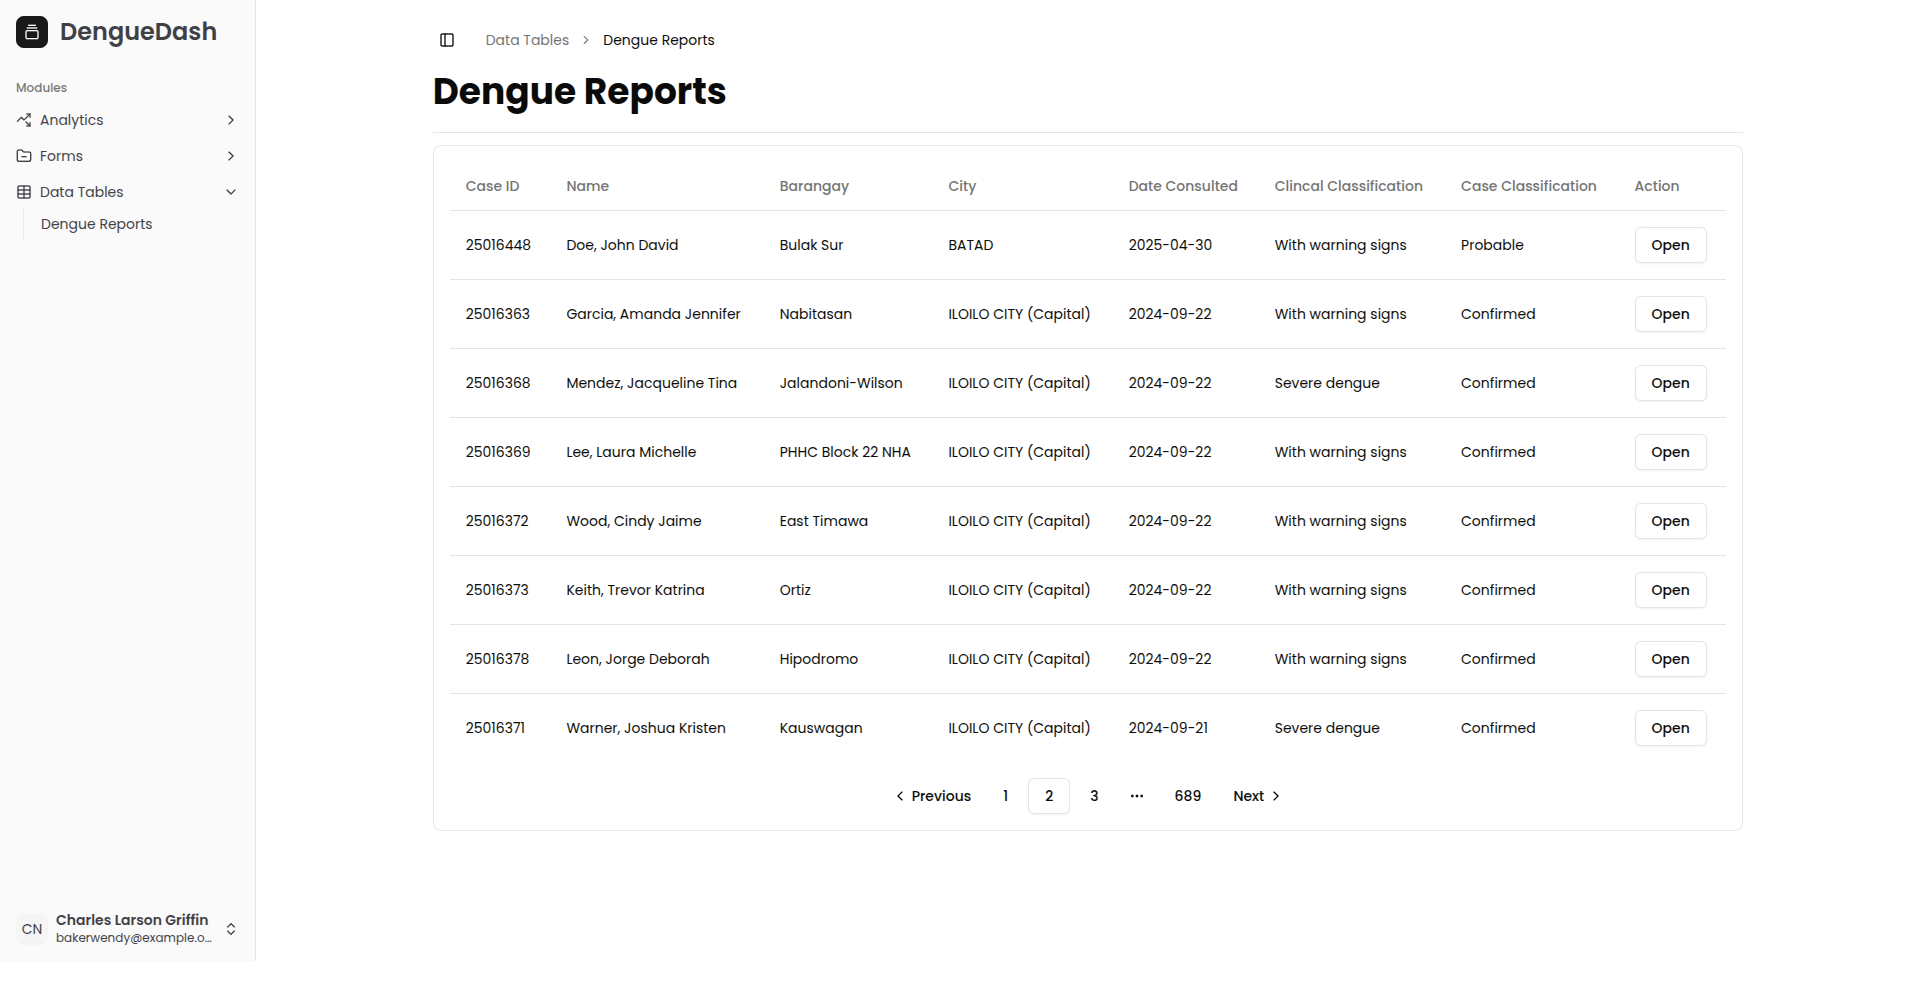
\includegraphics[width=1\textwidth]{dengue_reports}
	\caption{Dengue Reports}
	\label{fig:dengue_reports}
\end{figure}
\begin{figure}[H]
	\centering
	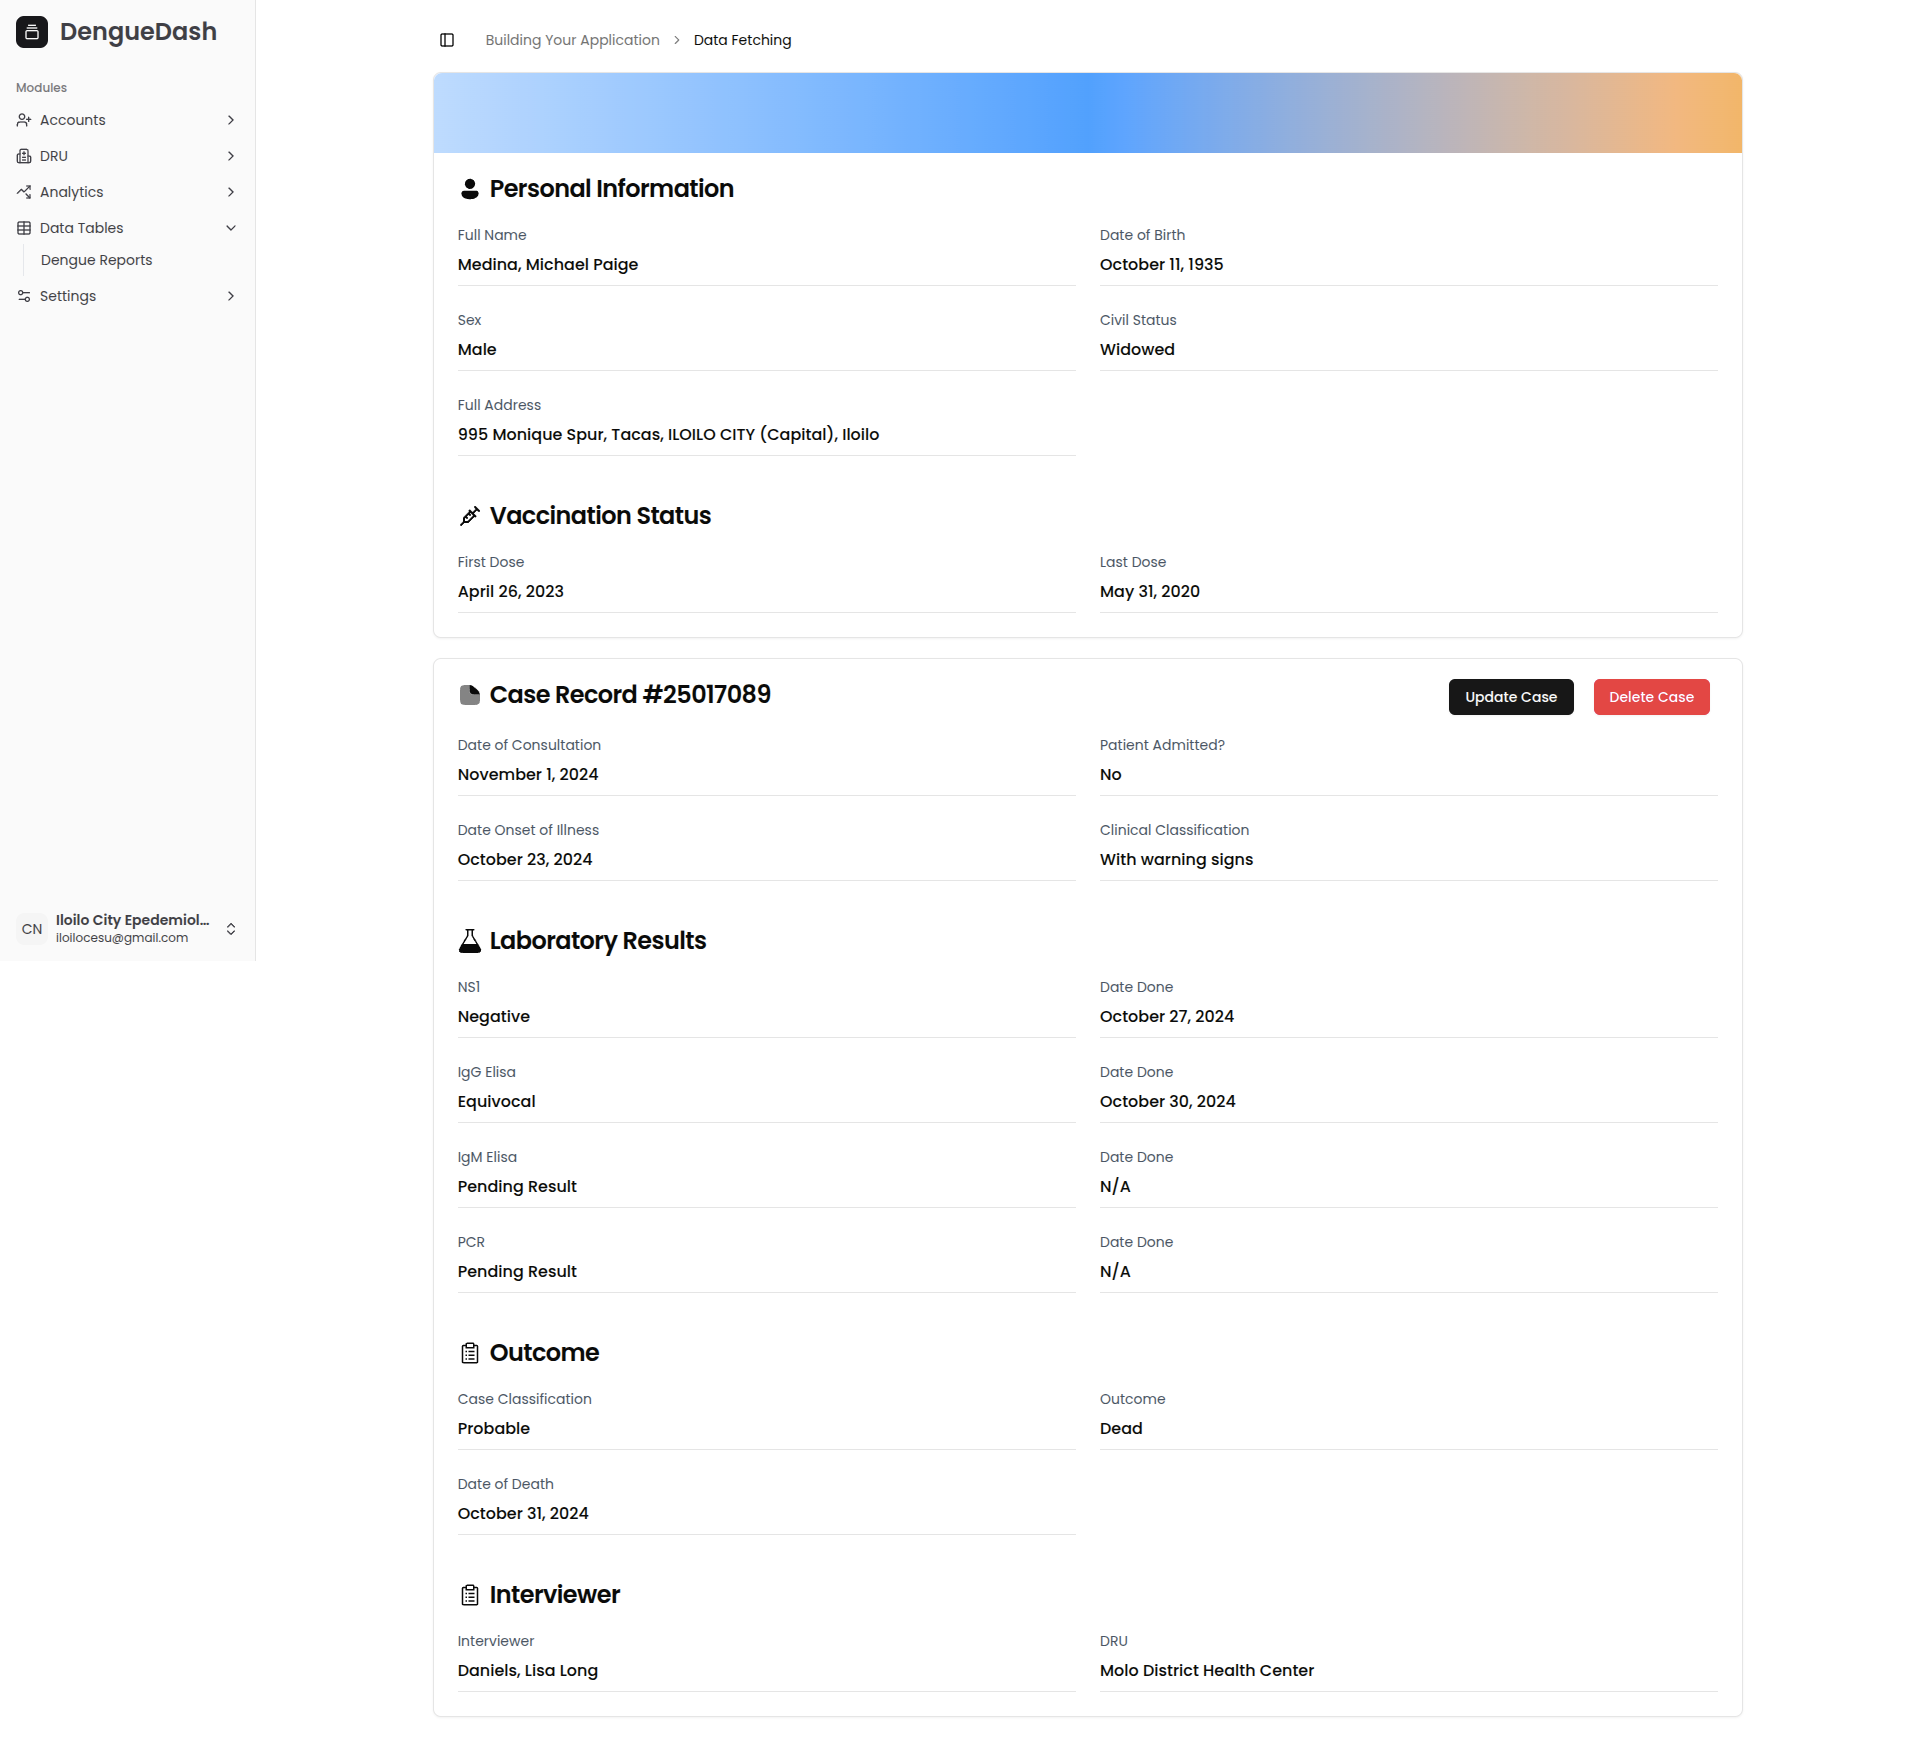
\includegraphics[width=1\textwidth]{detailed_case_report}
	\caption{Detailed Case Report}
	\label{fig:detailed_case_report}
\end{figure}

To update the case, the user can click the "Update Case" button, where a dialog will appear, and the updateable fields will be shown. It is worth noting that in this case, only fields under Laboratory Results and Outcome are included since they are the only ones that are time-based, where the result may change in the future. After updating, a prompt will show confirming the action of the user. Moving forward, to delete a case record, the user must click the "Delete Case" button, and a prompt verifying the action will appear. After confirming, the case will be deleted permanently.

\begin{figure}[H]
	\centering
	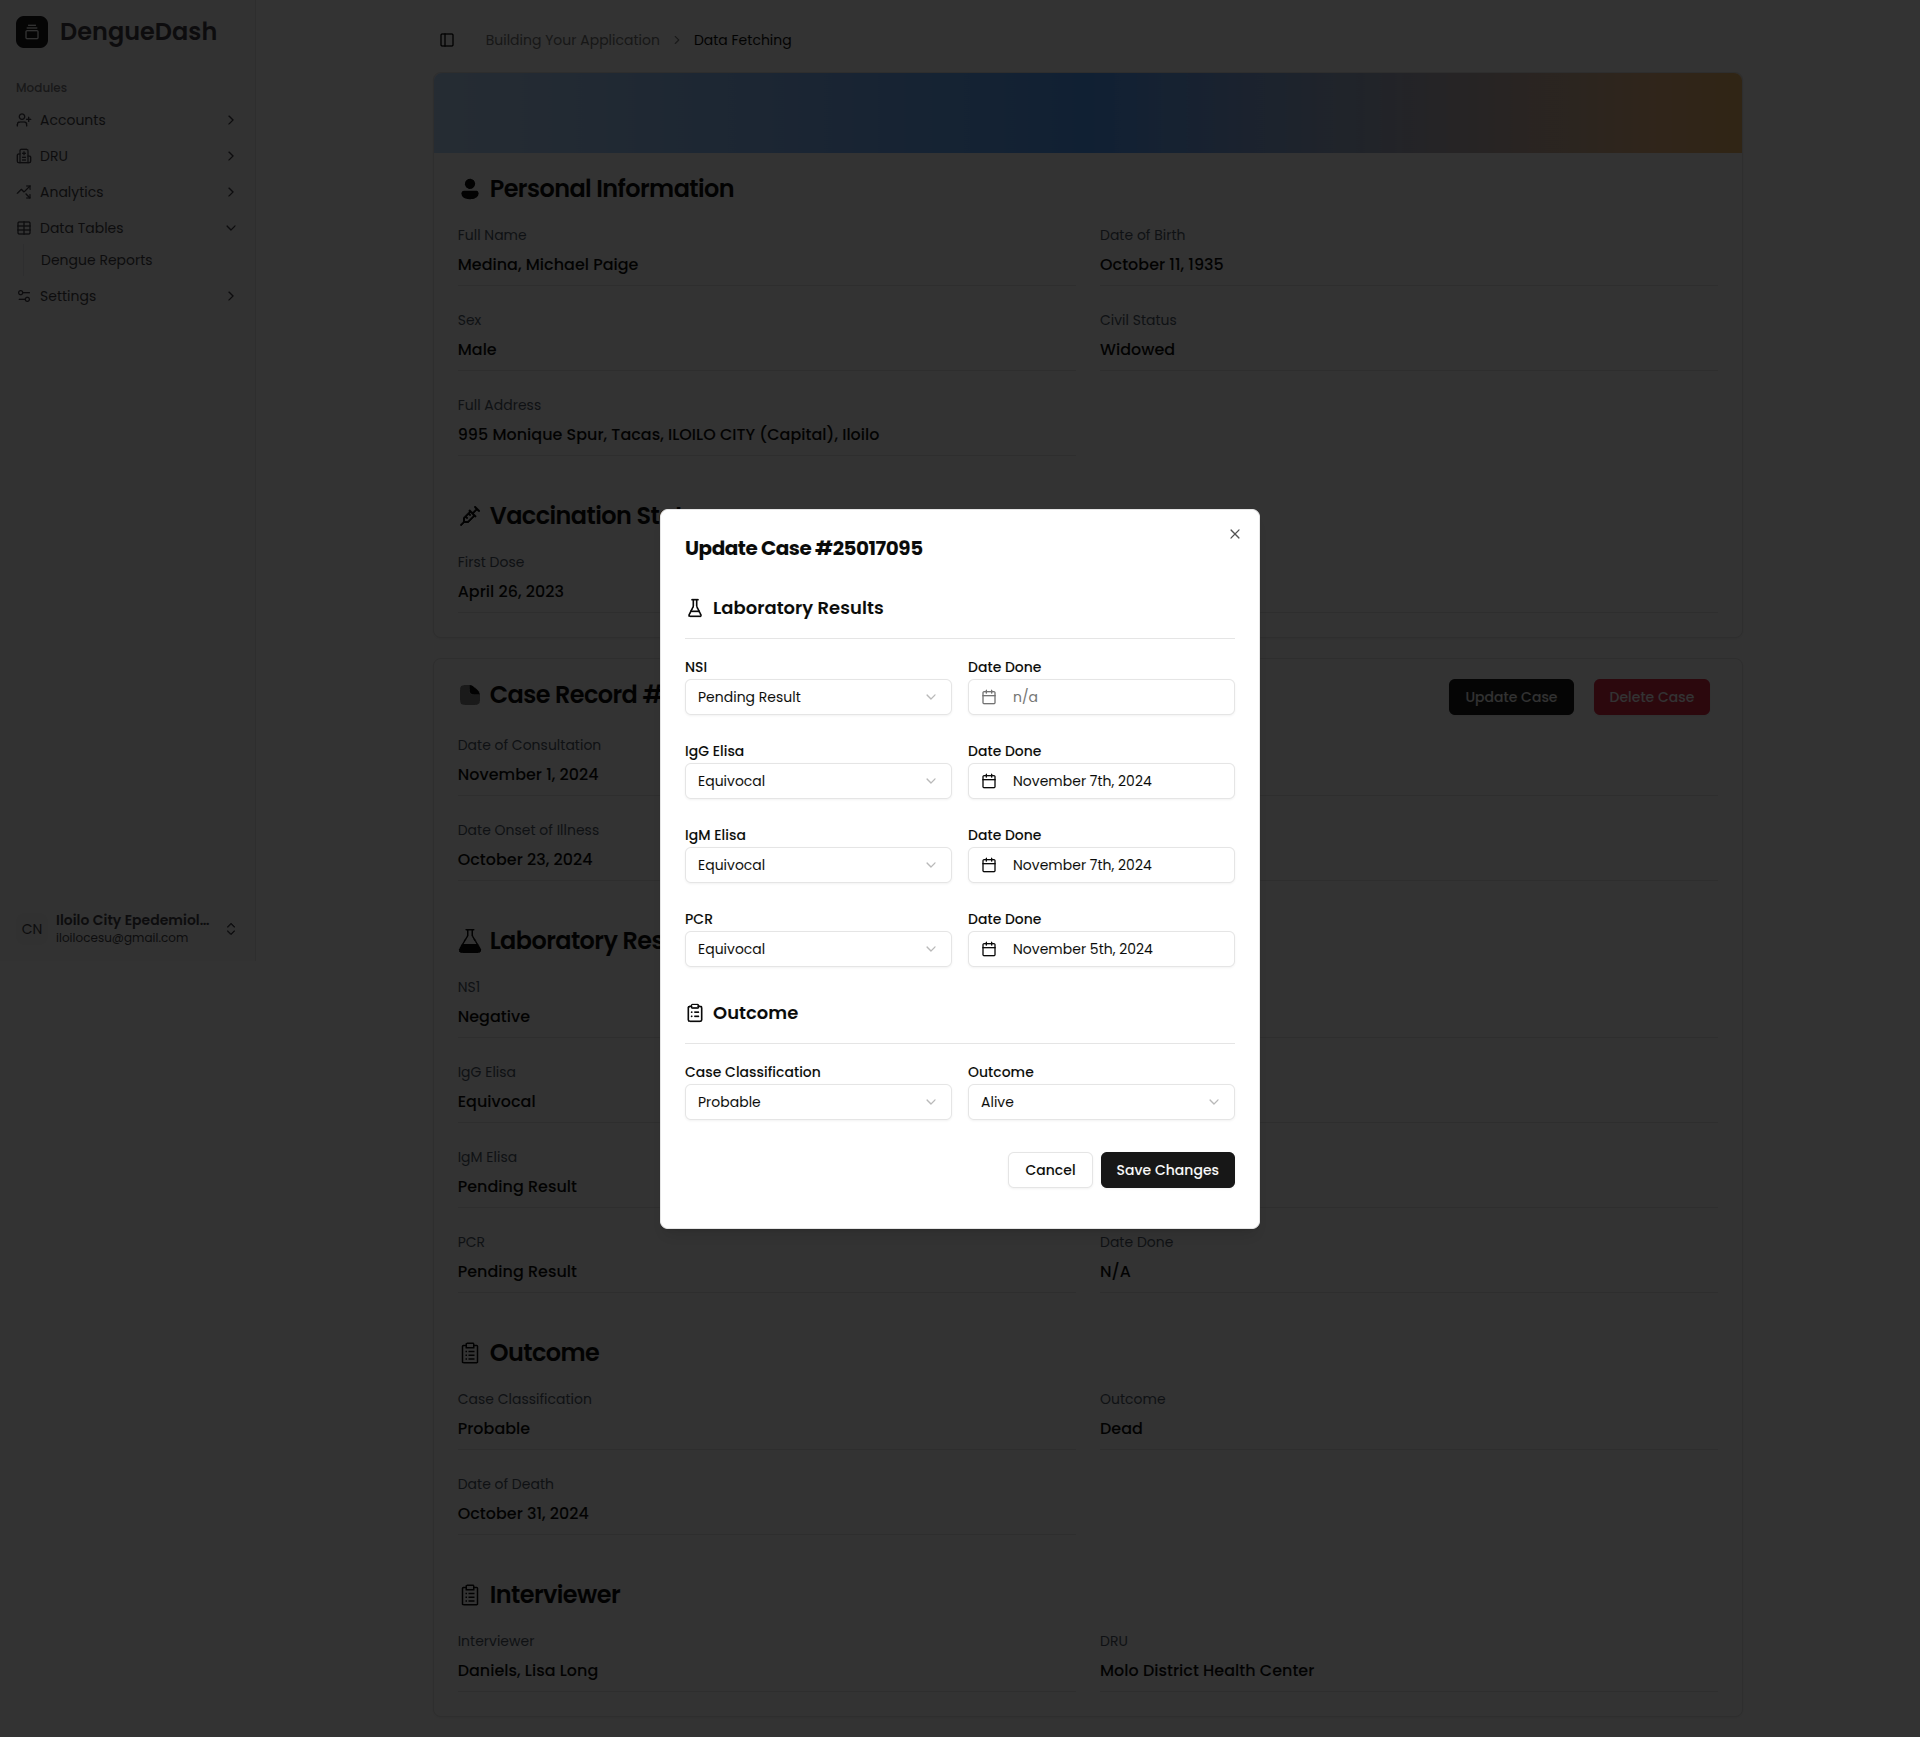
\includegraphics[width=1\textwidth]{update_report}
	\caption{Update Report Dialog}
	\label{fig:update_report}
\end{figure}
\begin{figure}[H]
	\centering
	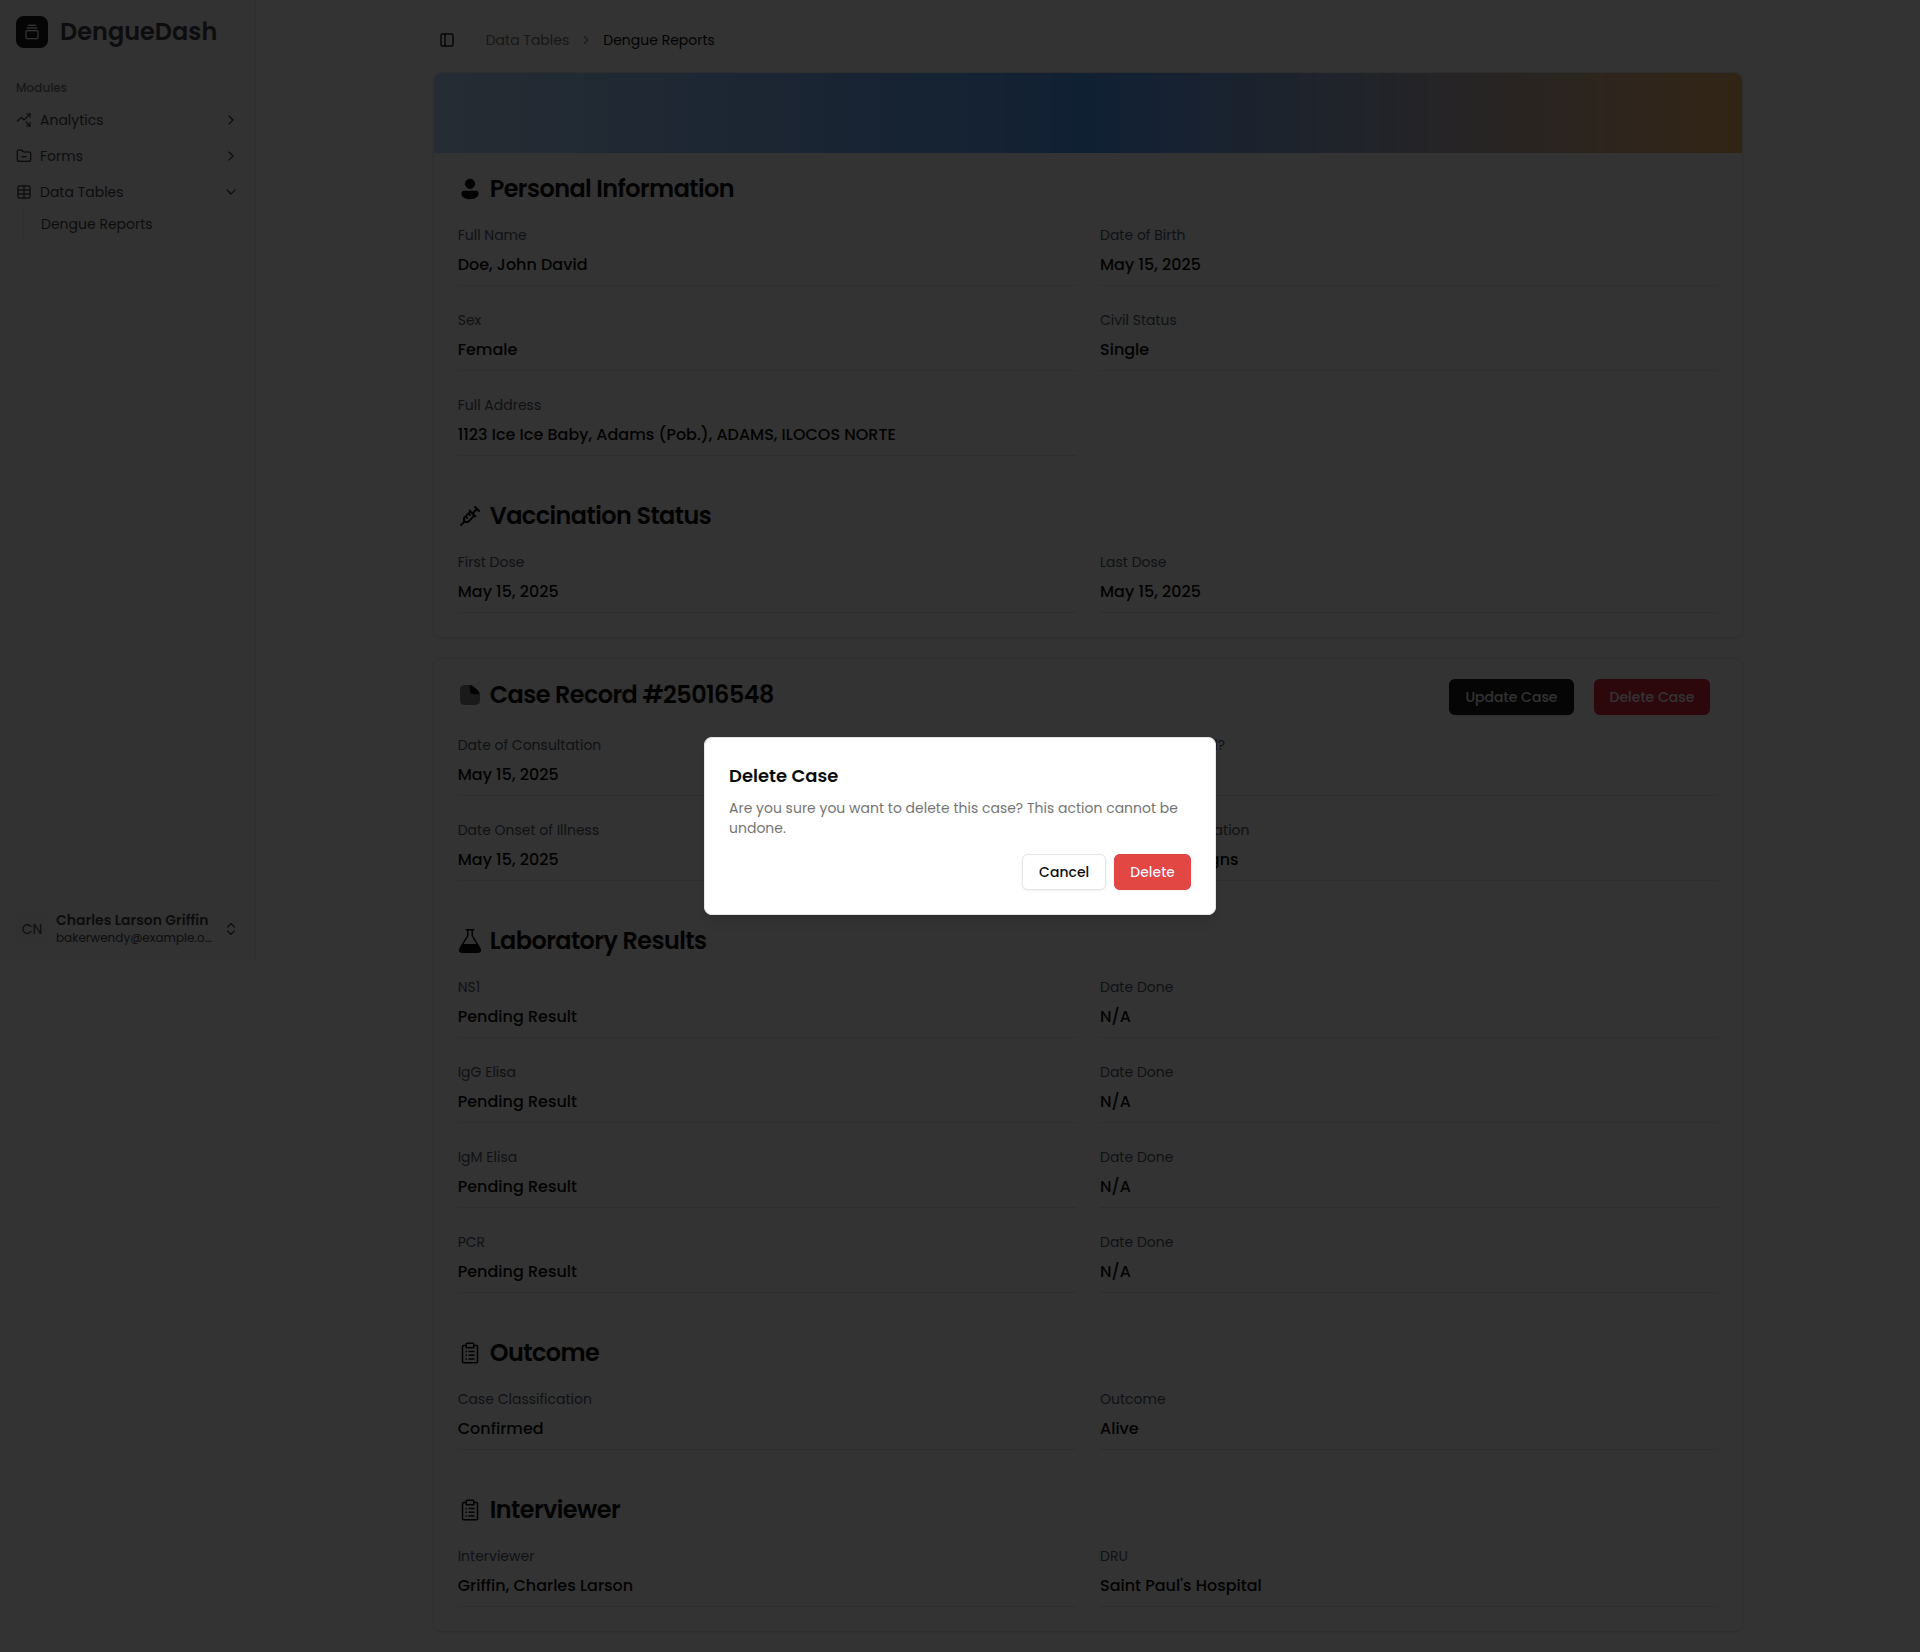
\includegraphics[width=1\textwidth]{delete_report}
	\caption{Delete Report Alert Dialog}
	\label{fig:delete_report}
\end{figure}

\subsubsection{Forecasting}

The main highlight of the web application's feature is the Forecasting Page. This is where users can forecast dengue cases for the next following weeks. To predict, the application utilizes the exported LSTM model in a Keras format derived from training the consolidated data from the database. It requires the recent weekly dengue cases, weather variable data (temperature, humidity, and rainfall) based on the window size, and future weather data through OpenWeatherMap API. However, due to limitations imposed in the current plan subscribed in the API, only the next 16 days of weather data can be fetched. As a result, the web application can only make a two-week prediction. Moving forward, the Forecasting page, as shown in Figure \ref{fig:forecasting}, introduces a user-friendly interface that shows the current cases for the week, and the predictions for the next two weeks with a range of 90 percent to 110 percent confidence interval that is presented in a simple but organized manner. There is also a line chart that shows the number of cases from the last 5 weeks plus the forecasted weekly cases. In addition, the current weather data for a specific week is also shown as well as the the forecasted weather data fetched from the said API. Lastly, locations where dengue cases have been reported for the current week are listed in the Location Risk Assessment component. 

\begin{figure}[H]
	\centering
	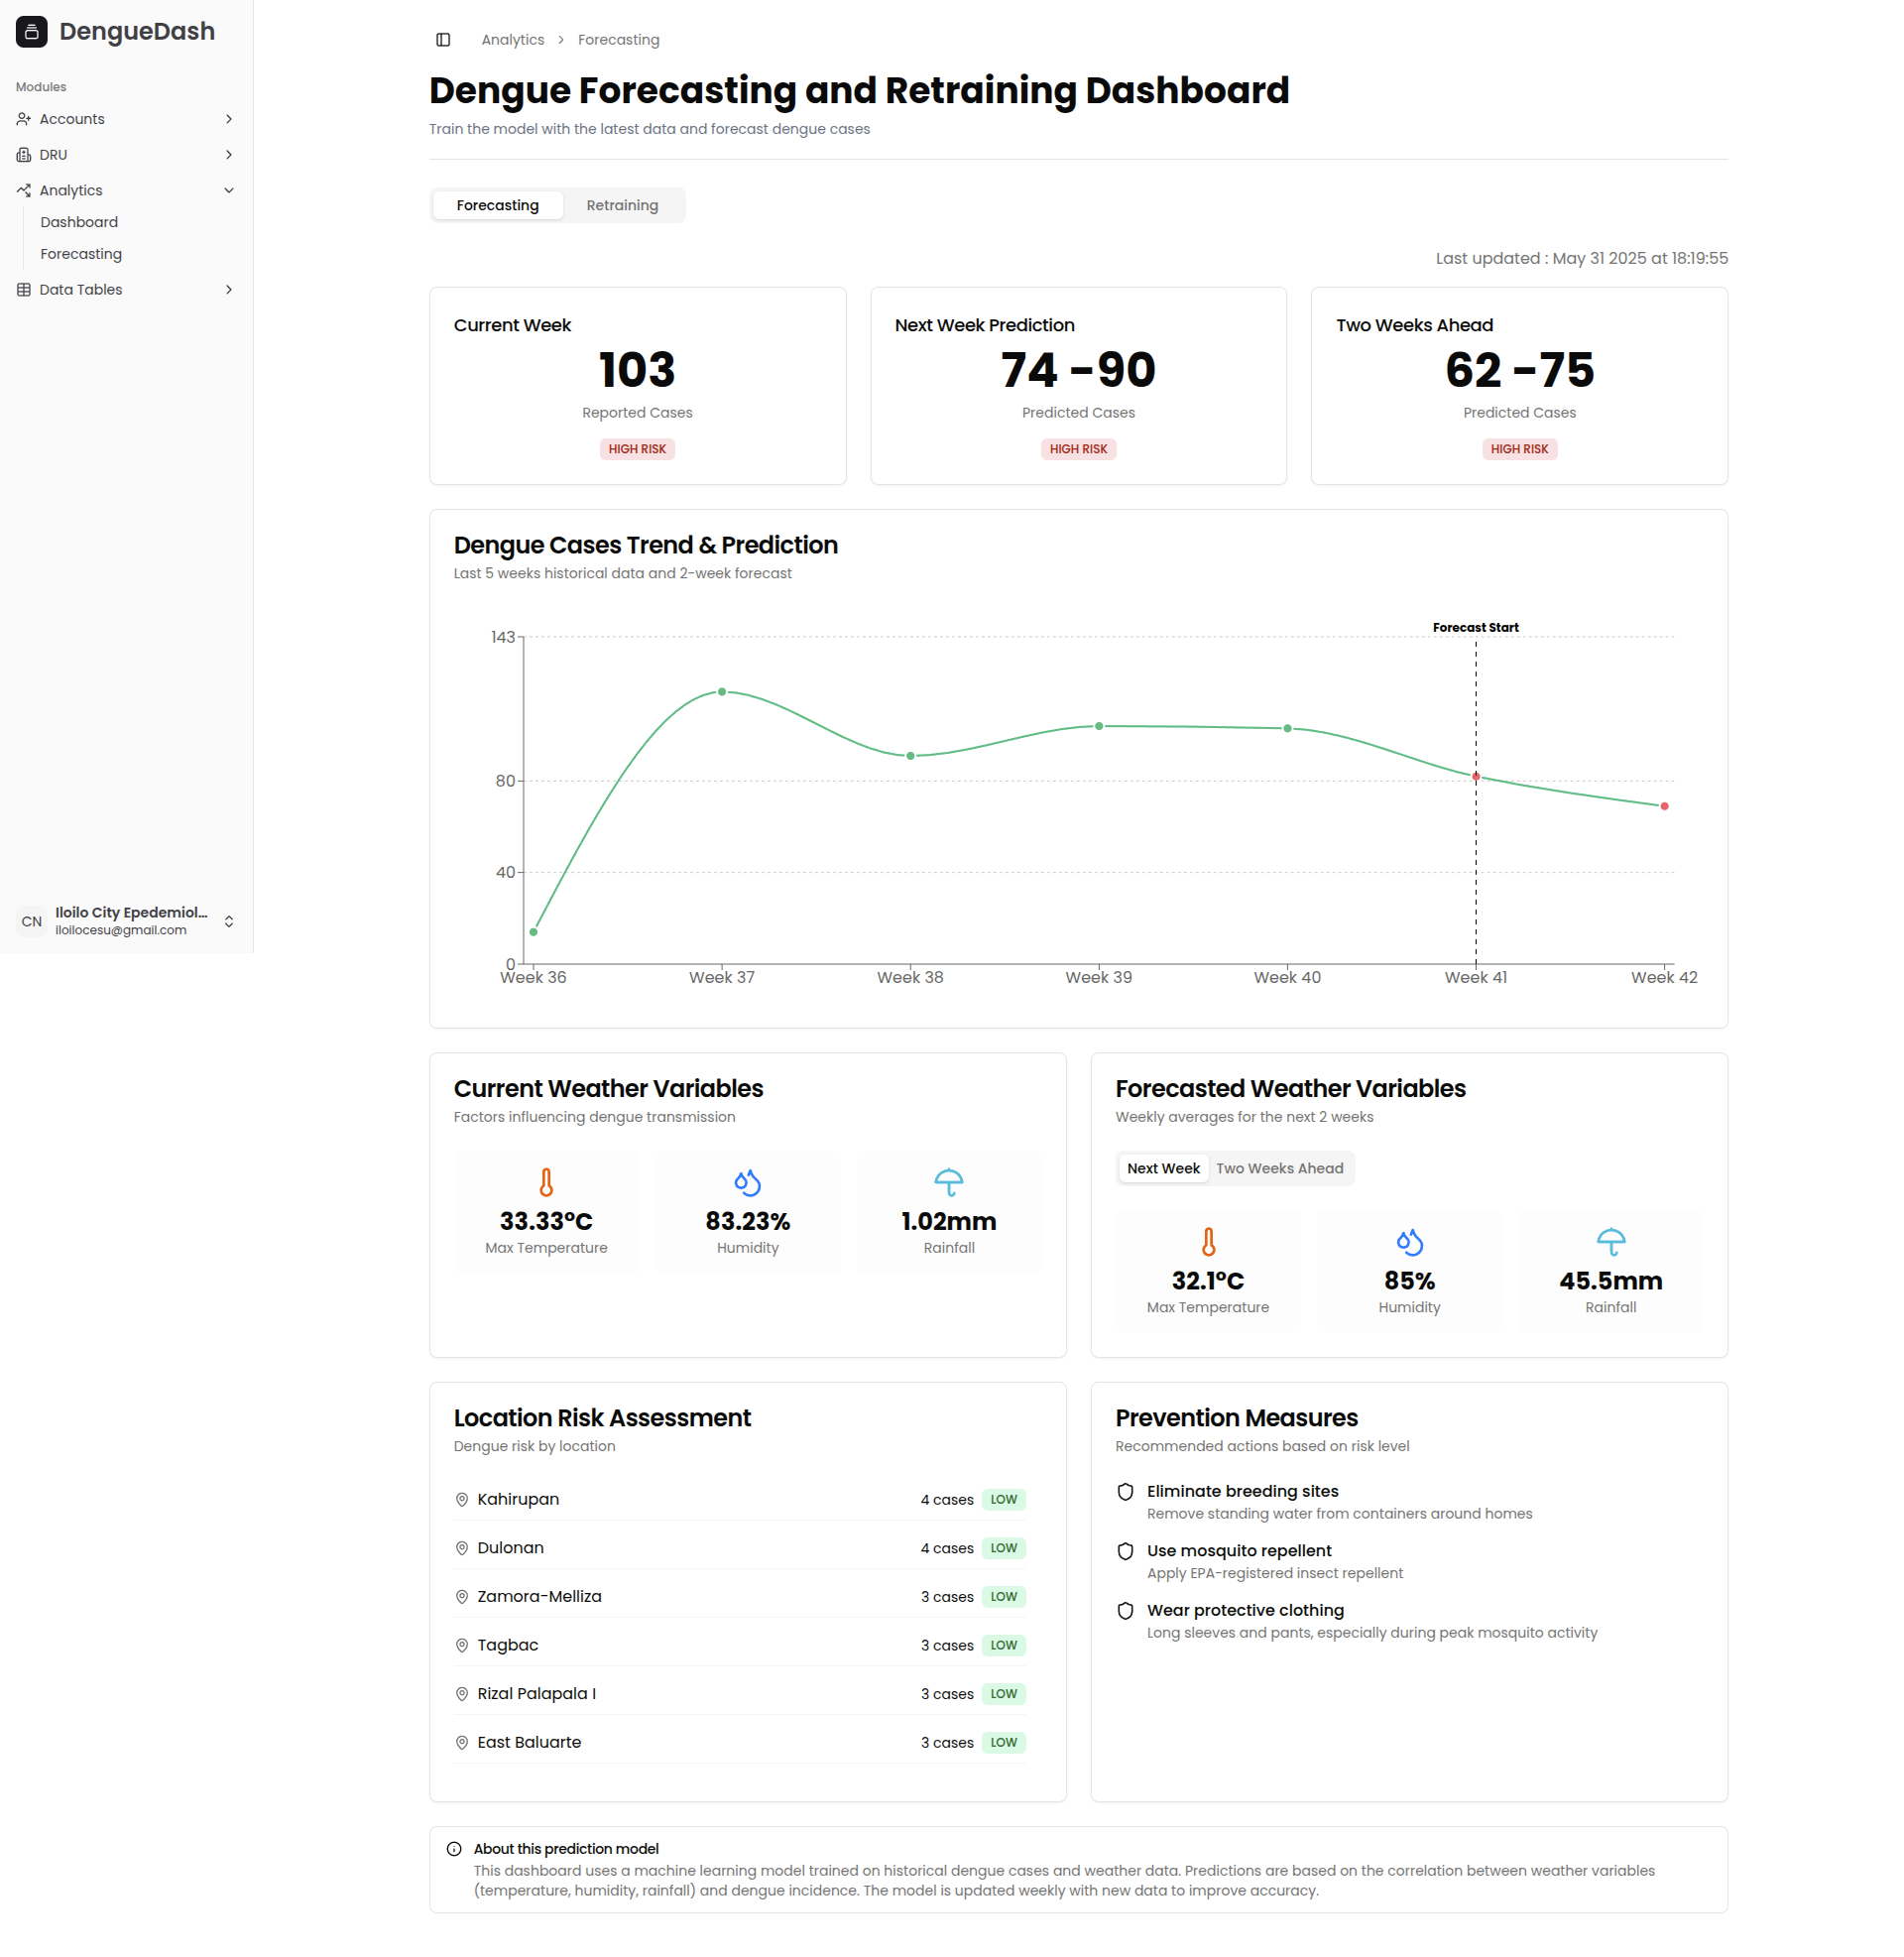
\includegraphics[width=1\textwidth]{forecasting}
	\caption{Forecasting Page}
	\label{fig:forecasting}
\end{figure}

\subsection{Admin Interface}

\subsubsection{Retraining}

With LSTM being the best-performing model among the models used in forecasting dengue cases, it is the model chosen to power the prediction and retraining of the consolidated data within the web application. Since the retraining process consumes a lot of processing power and requires a more advanced understanding of how it works, it was decided that the said feature should only be available to admin users. Furthermore, the retraining component in the Forecasting page includes three additional components that include the configuration of LSTM parameters (Figure \ref{fig:retraining_configs}), the actual retraining of the consolidated data from the database (Figure \ref{fig:retraining_train}), and the results of the retraining that shows the current and previous model metrics depending on the parameters entered (Figure \ref{fig:retraining_results}). It is also worth noting that when trained, the model used a seeded number to promote reproducibility. 

\begin{figure}[H]
	\centering
	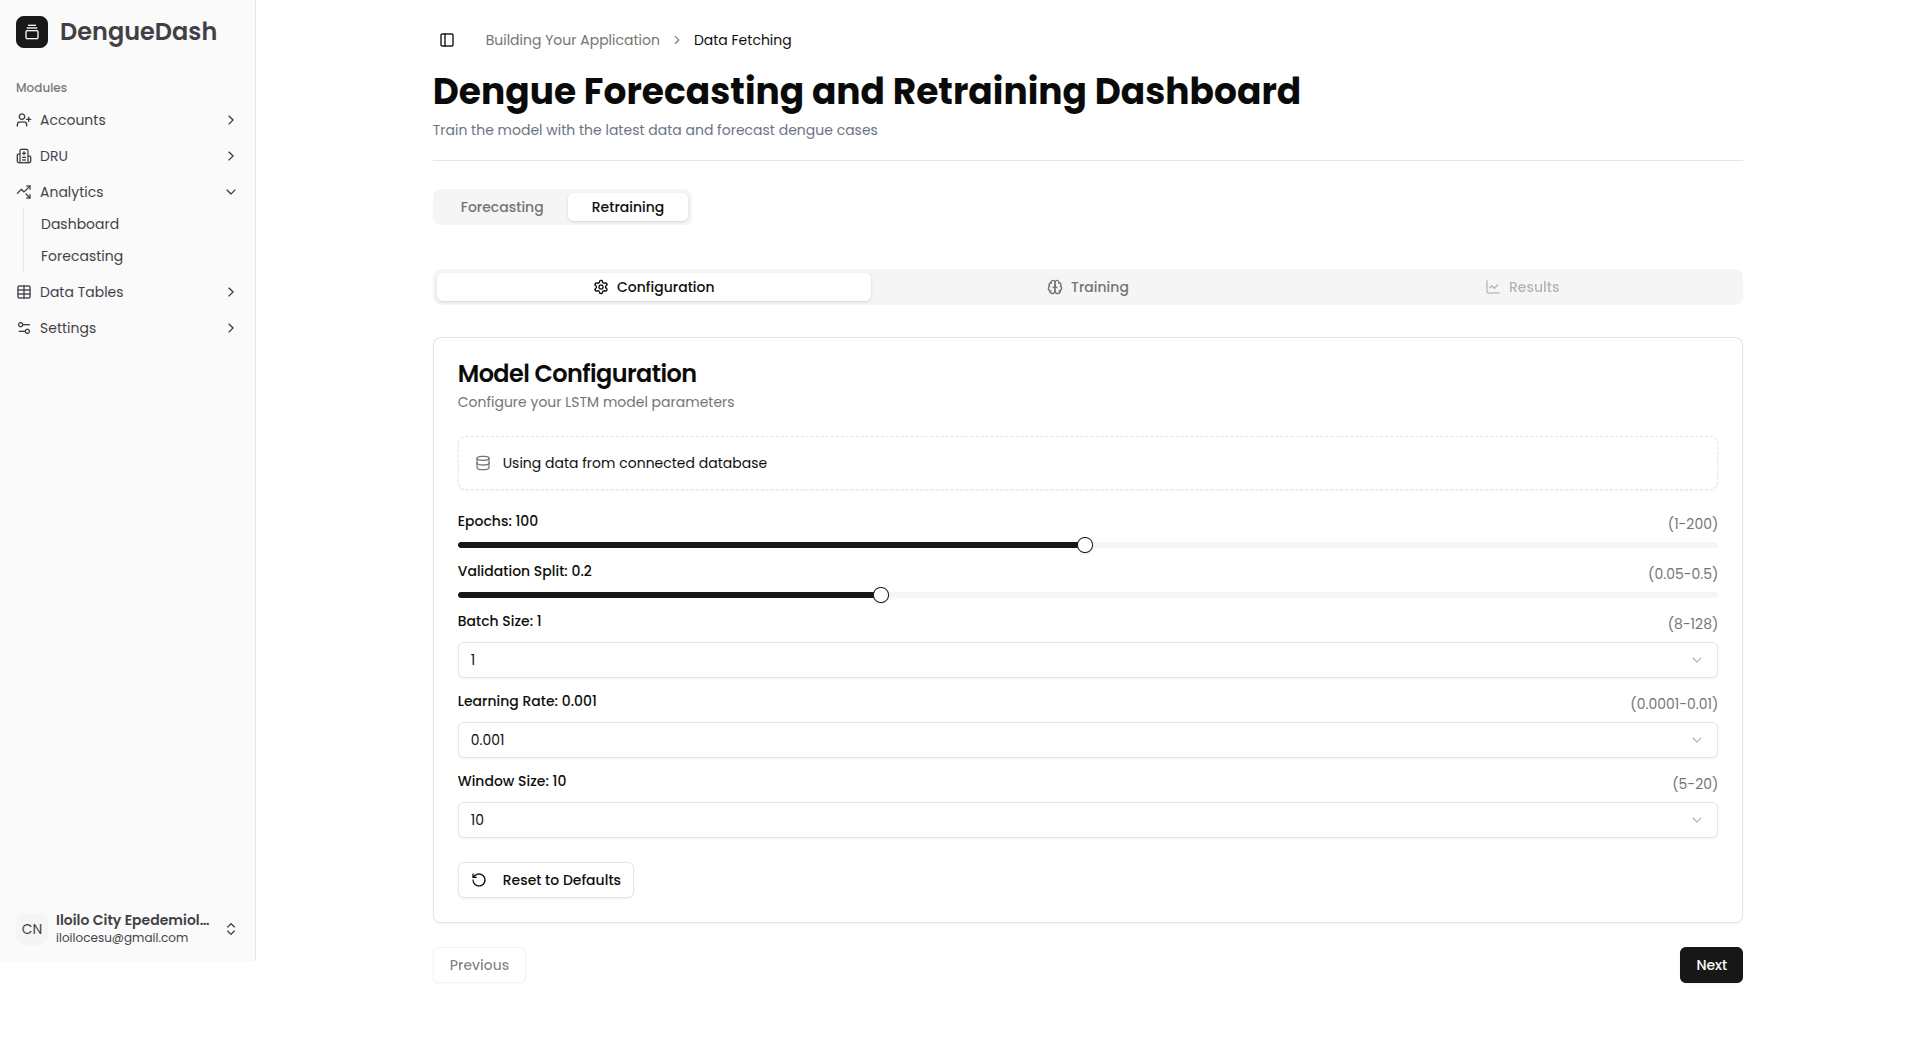
\includegraphics[width=1\textwidth]{retraining_configs}
	\caption{Retraining Configurations}
	\label{fig:retraining_configs}
\end{figure}
\begin{figure}[H]
	\centering
	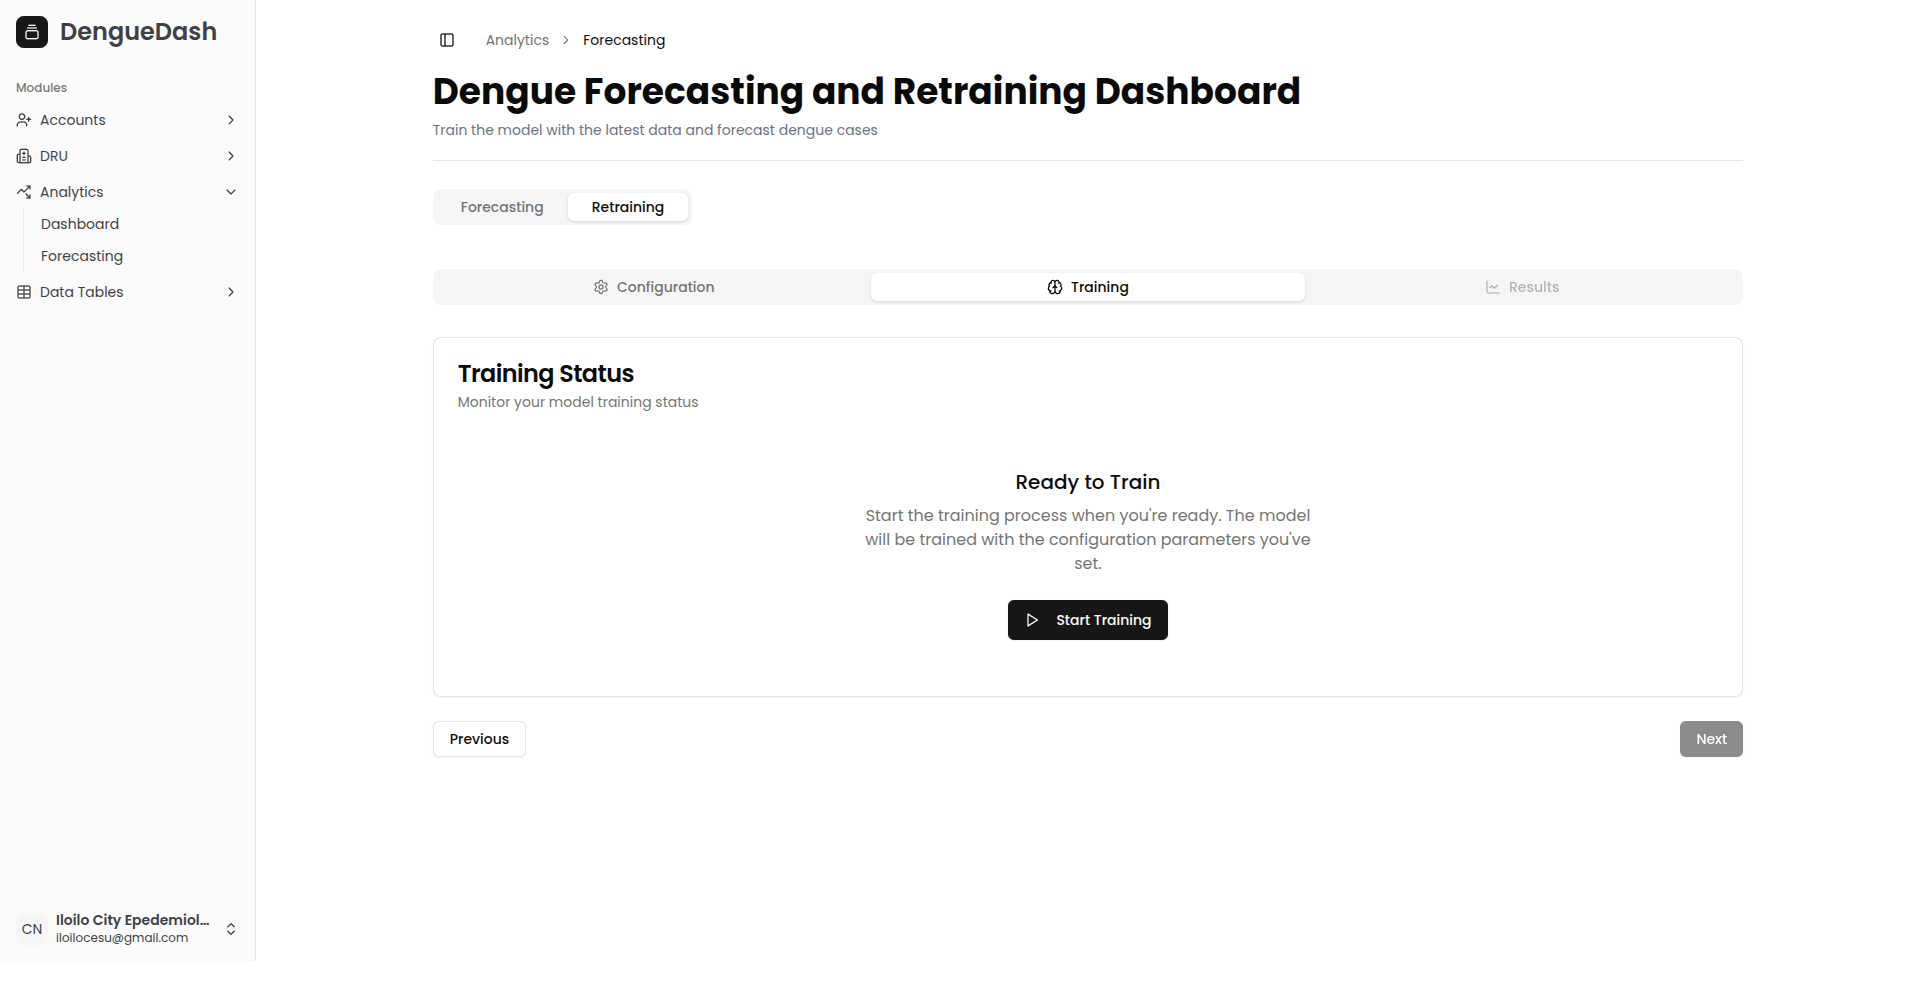
\includegraphics[width=1\textwidth]{retraining_train}
	\caption{Start Retraining}
	\label{fig:retraining_train}
\end{figure}
\begin{figure}[H]
	\centering
	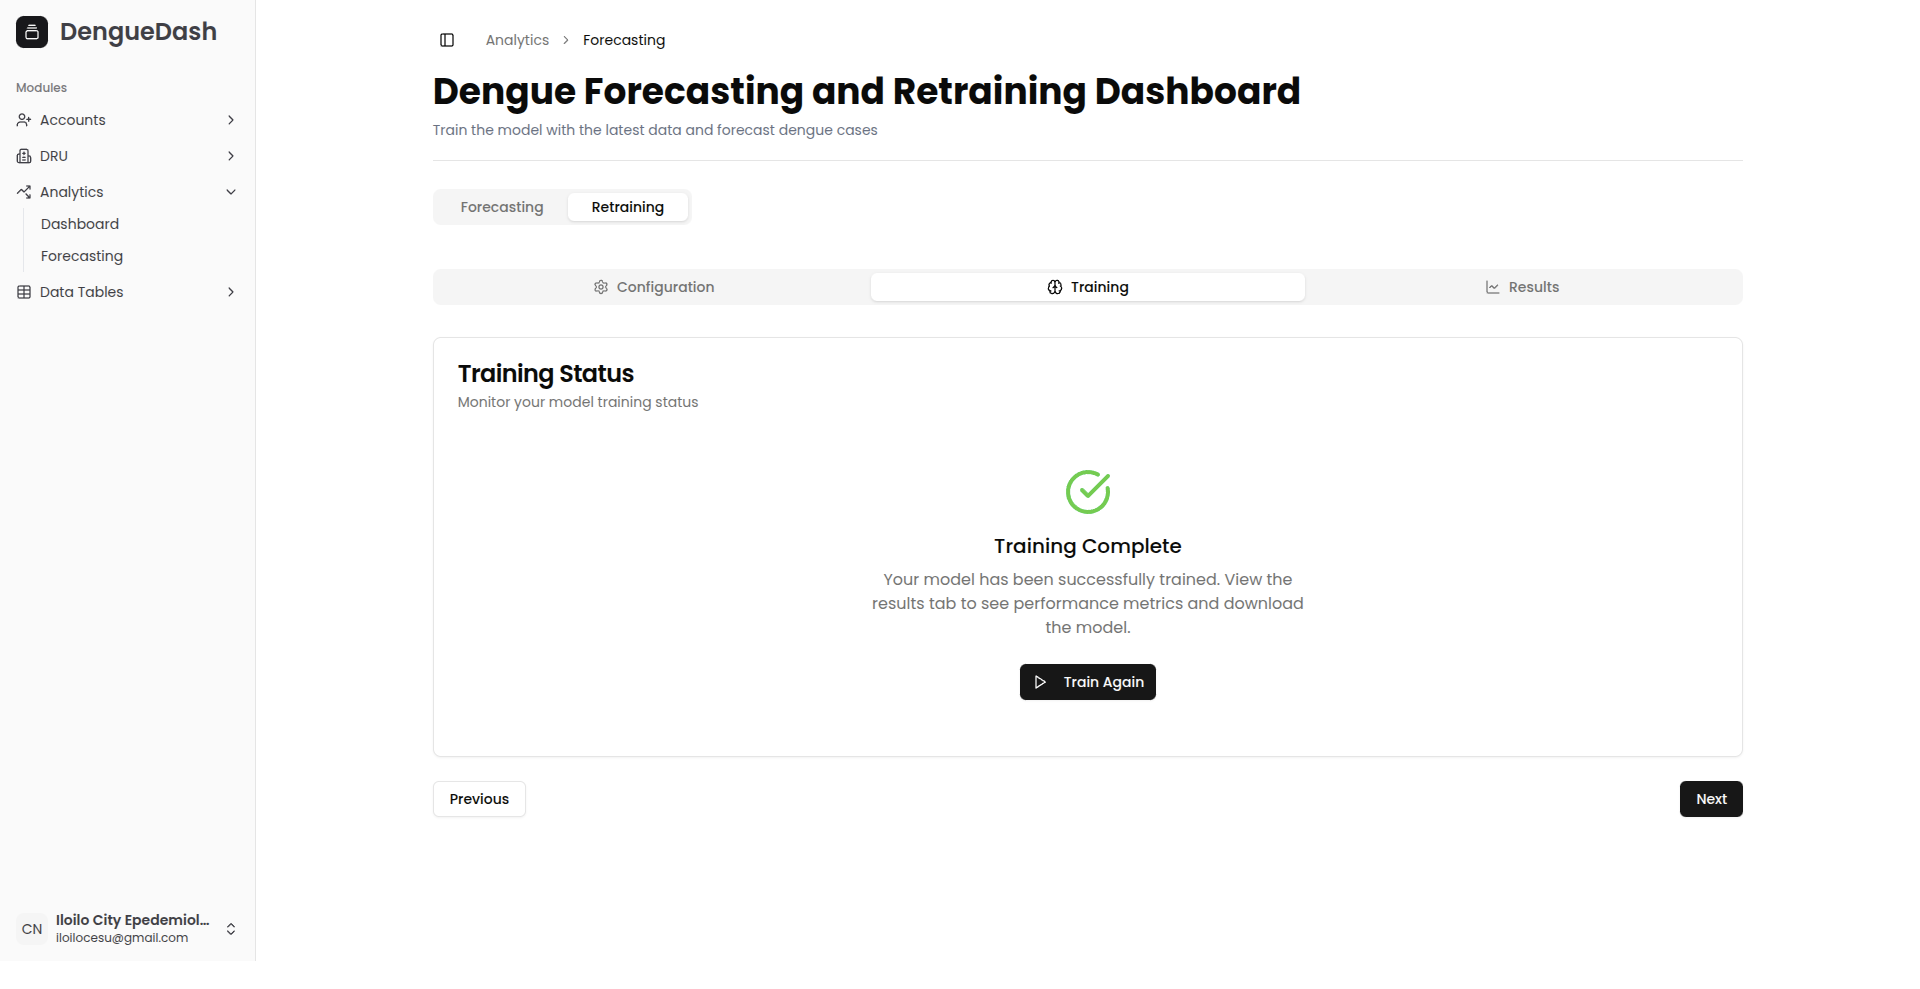
\includegraphics[width=1\textwidth]{retraining_results}
	\caption{Retraining Results}
	\label{fig:retraining_results}
\end{figure}

\clearpage

\subsubsection{Managing Accounts}

Proper management of accounts is important to protect the integrity and confidentiality of data. Thus, it is crucial for administrators to track their users and control the flow of information. As discussed in the user registration of encoders, admin users from a specific DRU or surveillance have the power to grant them access to the web application. Figure \ref{fig:pending_accounts} illustrates the interface for this scenario, as the admins can approve or reject their applications. Once approved, these users can access the features given to encoders and may be promoted to have administrative access, as shown in Figure \ref{fig:account_details}. When deleting an account, the user's email will be blacklisted and illegible to use when creating another account, and all the cases reported by this user will be soft-deleted. The same figure also shows the expanded details of the user, which include personal information and brief activity details within the system.

\begin{figure}[H]
	\centering
	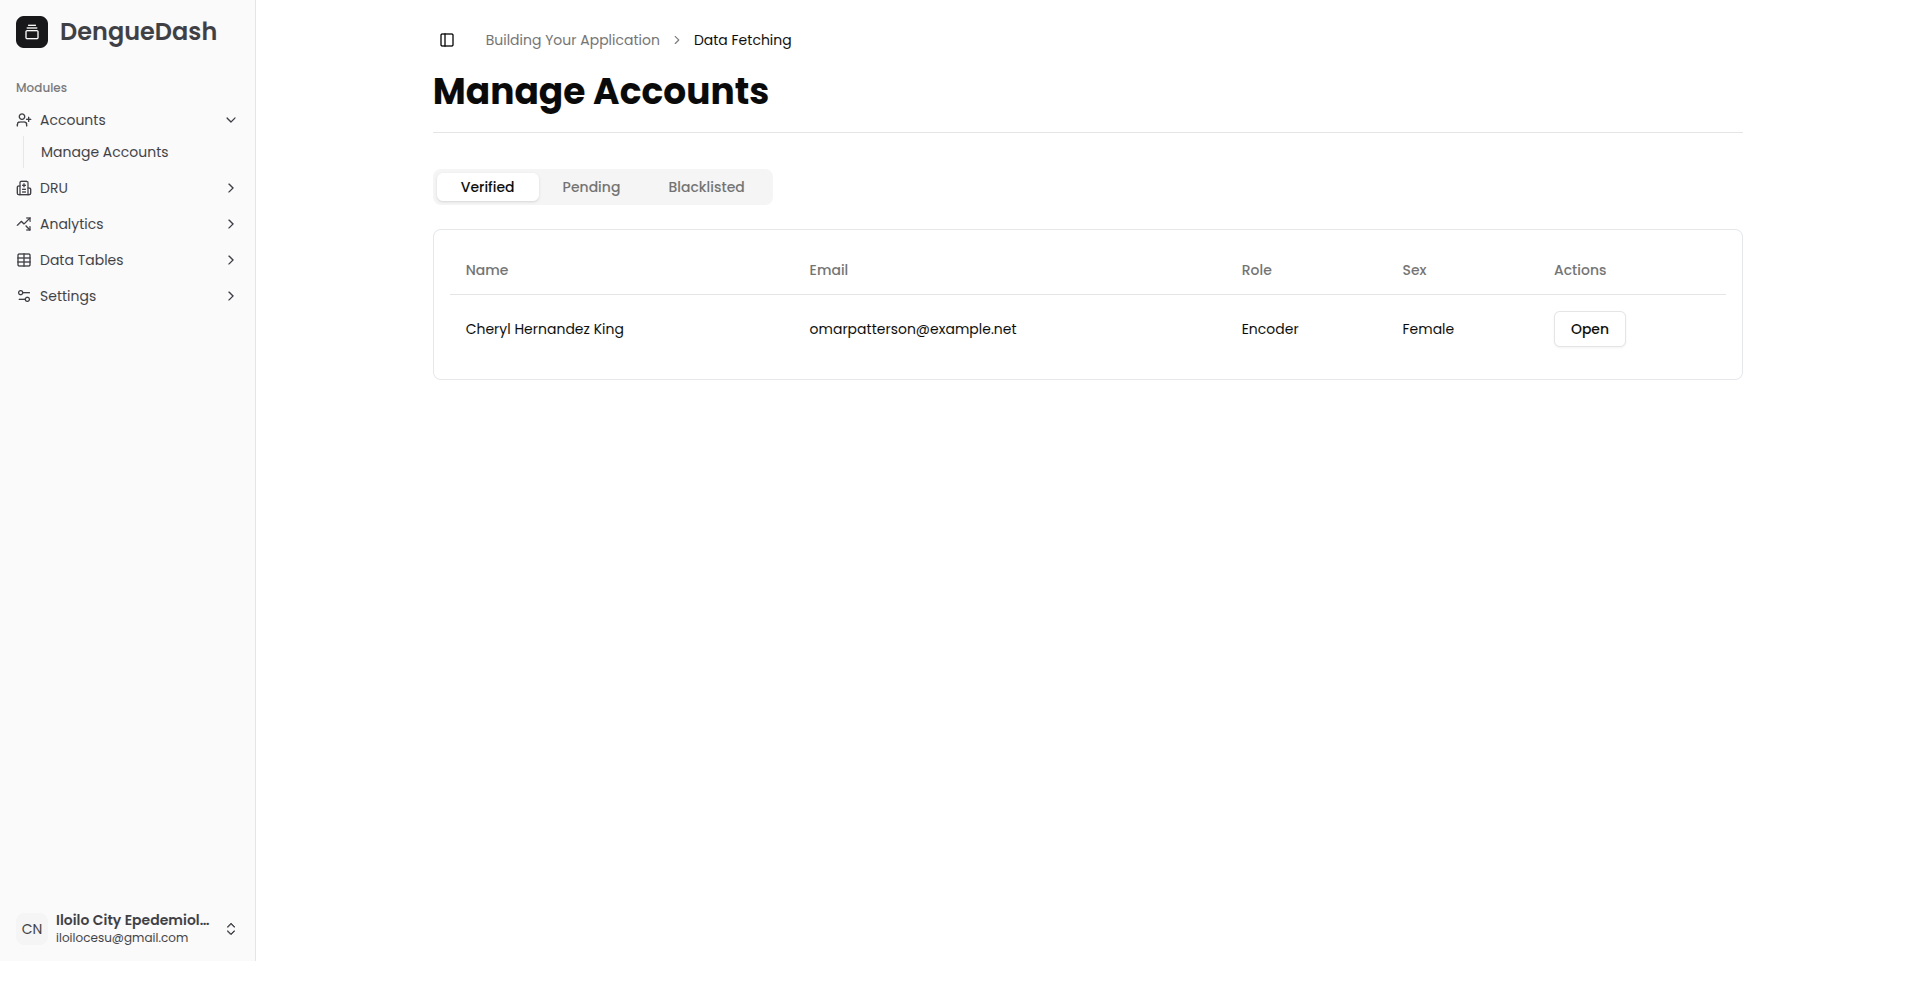
\includegraphics[width=1\textwidth]{verified_accounts}
	\caption{List of Verified Accounts}
	\label{fig:verified_accounts}
\end{figure}
\begin{figure}[H]
	\centering
	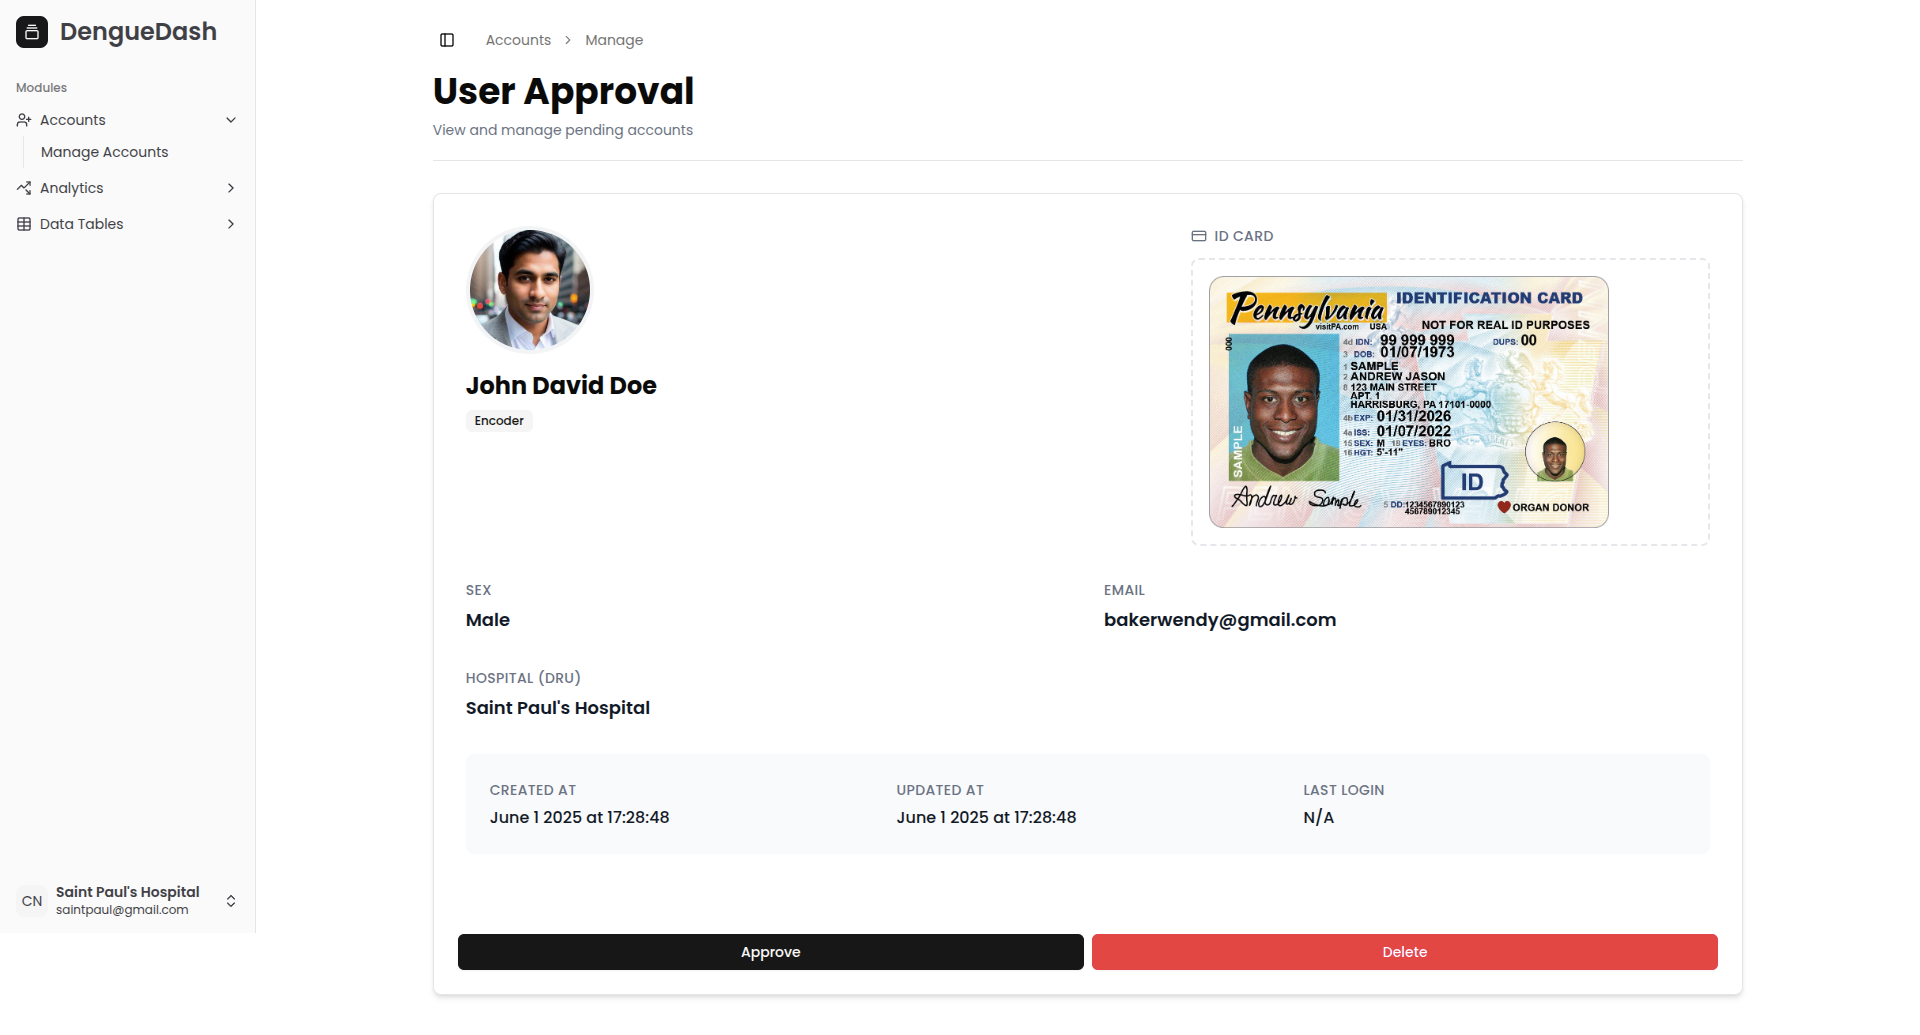
\includegraphics[width=1\textwidth]{pending_accounts}
	\caption{List of Pending Accounts}
	\label{fig:pending_accounts}
\end{figure}
\begin{figure}[H]
	\centering
	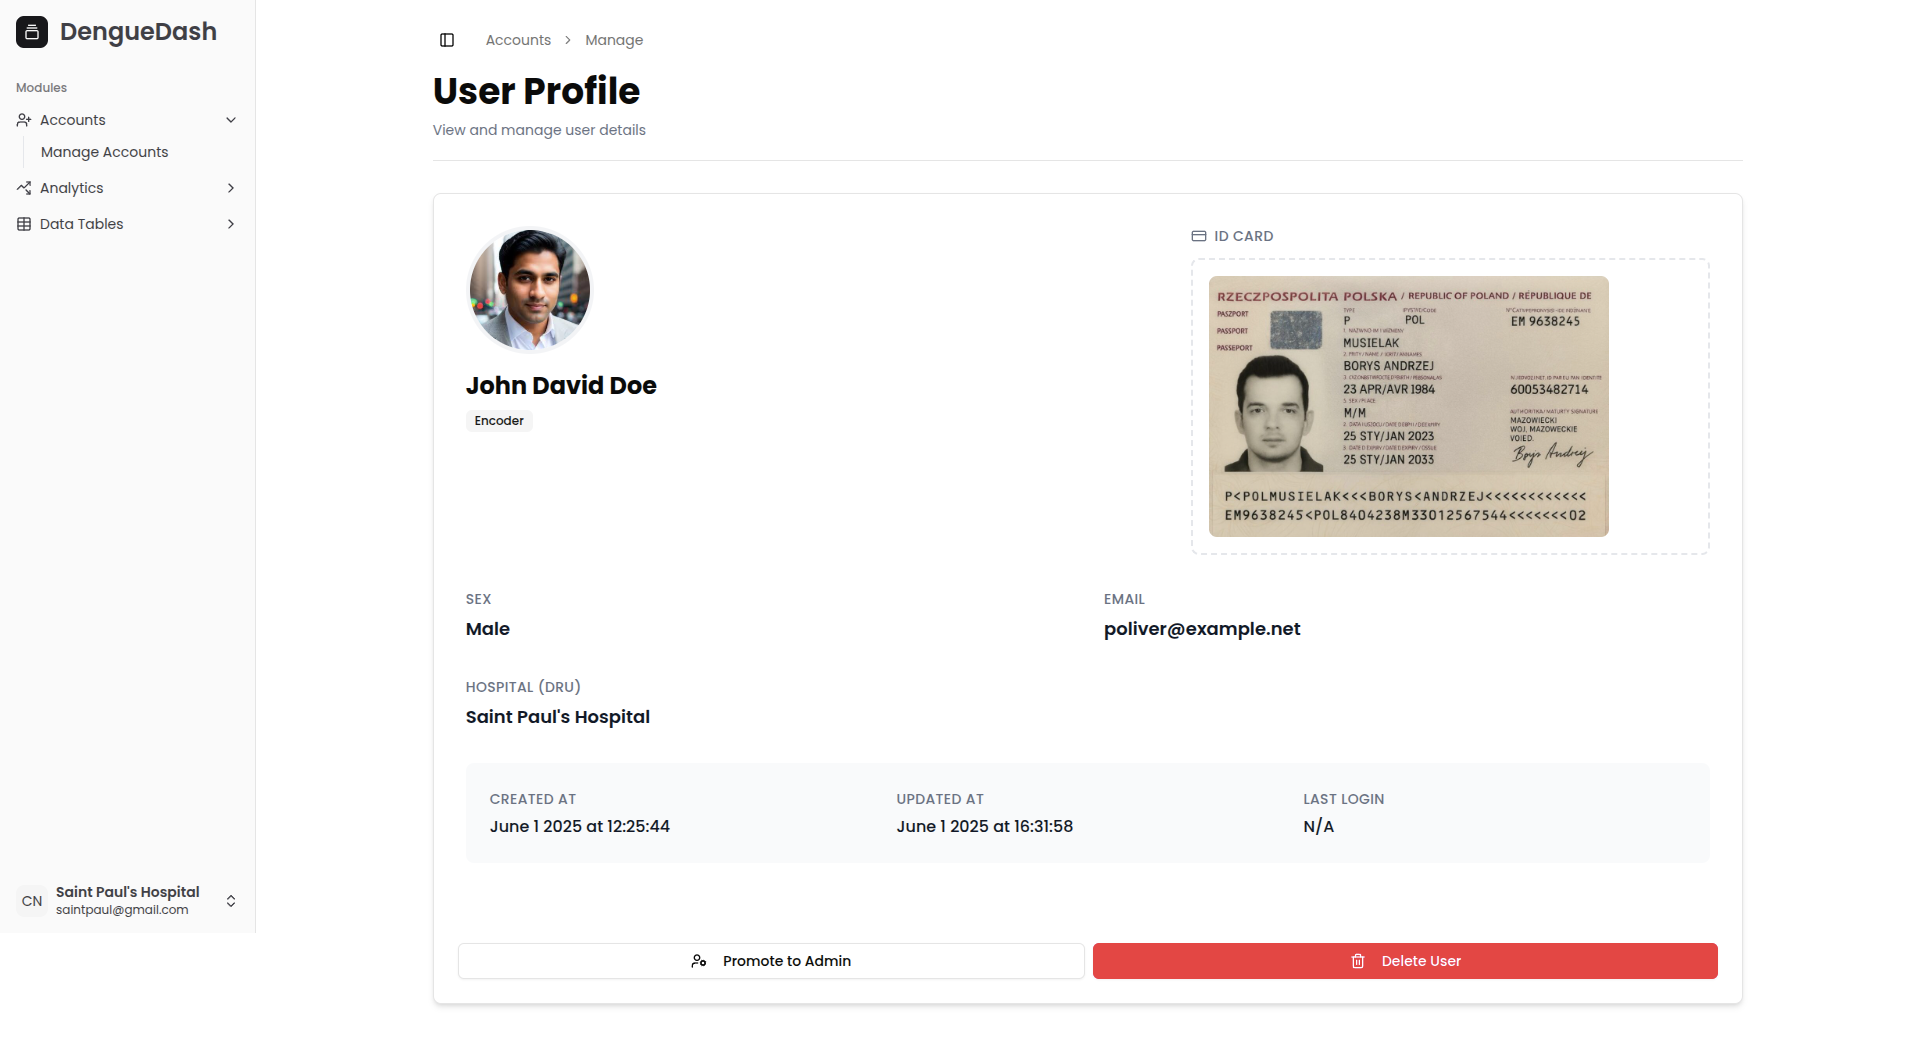
\includegraphics[width=1\textwidth]{account_details}
	\caption{Account Details}
	\label{fig:account_details}
\end{figure}

\subsubsection{Managing DRUs}

Unlike the registration of encoder accounts, the creation of Disease Reporting Units can only be done within the web application, and the user performing the creation must be an administrator of a surveillance unit. Figure \ref{fig:register_dru} presents the fields the admin user must fill out, and once completed, the new entry will show as being managed by that unit, as shown in Figure \ref{fig:browse_drus}. Figure \ref{fig:dru_details}, on the other hand, shows the details provided in the registration form as well as its creation details. There is also an option to delete the DRU, and when invoked, all the accounts being managed by it, and the cases reported under those accounts will be soft-deleted.

\begin{figure}[H]
	\centering
	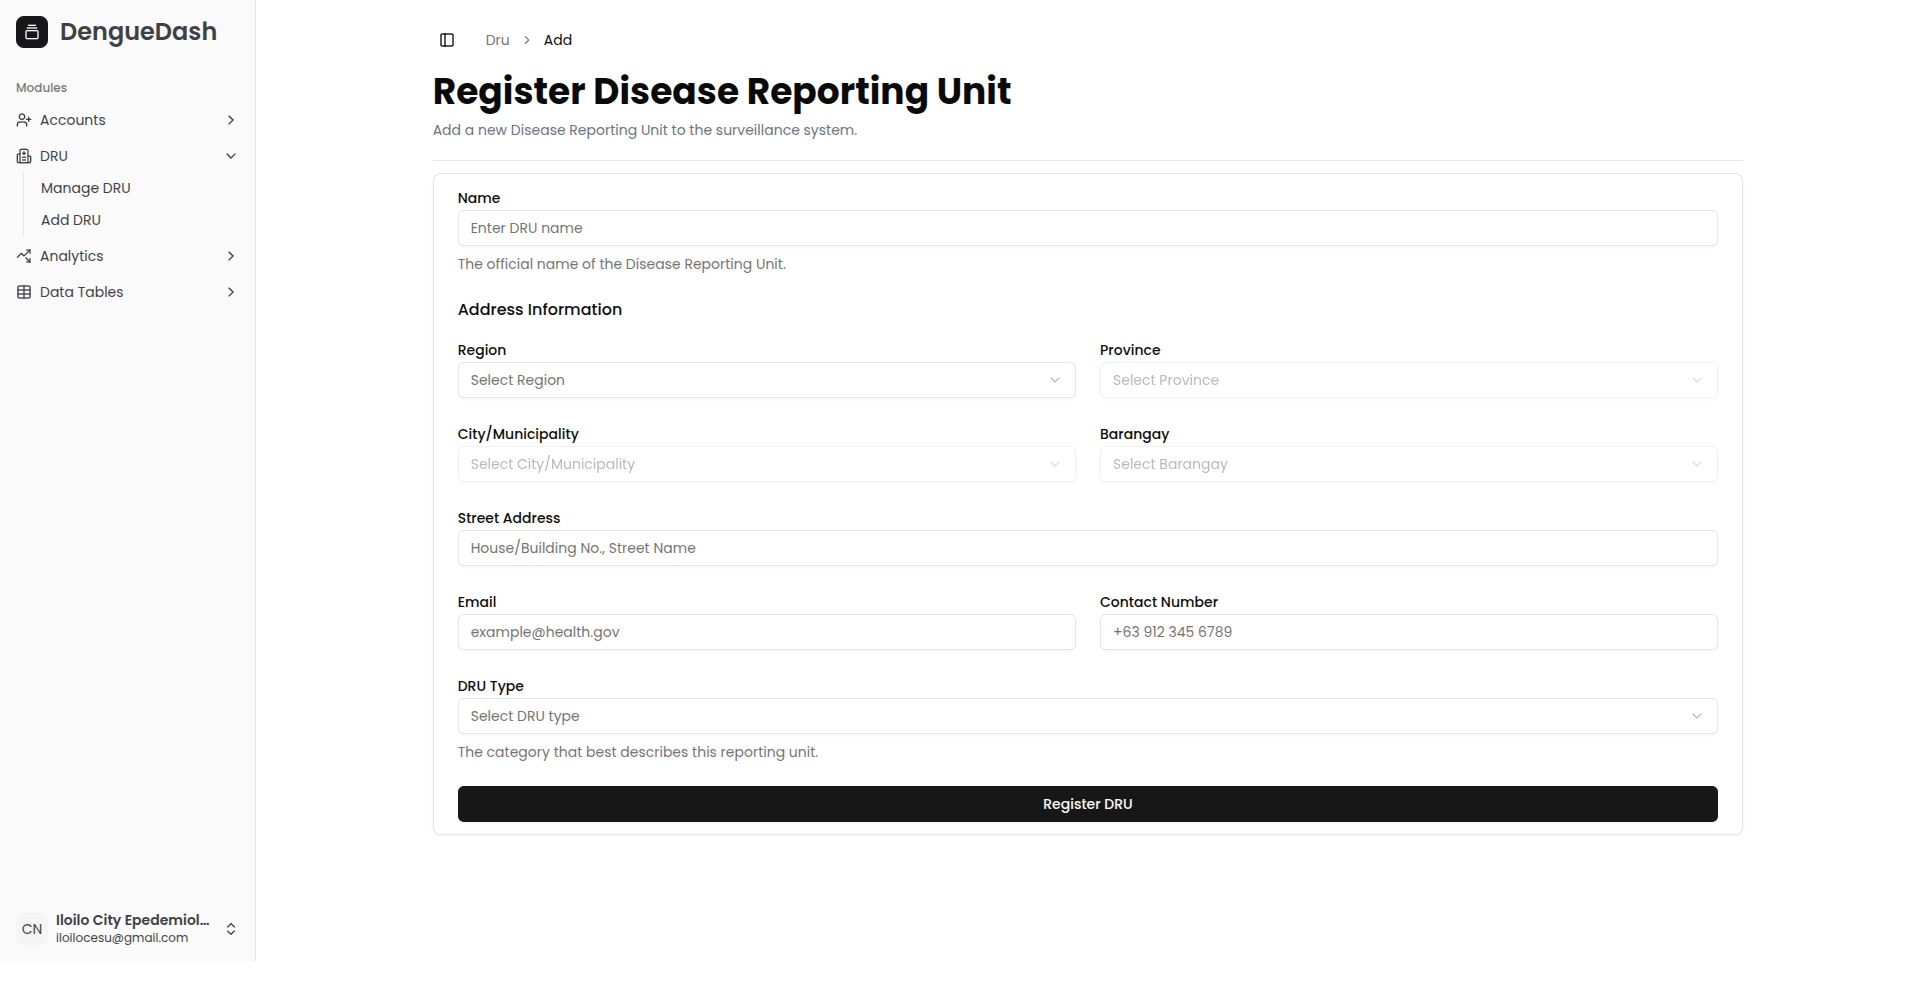
\includegraphics[width=1\textwidth]{register_dru}
	\caption{DRU Registration}
	\label{fig:register_dru}
\end{figure}
\begin{figure}[H]
	\centering
	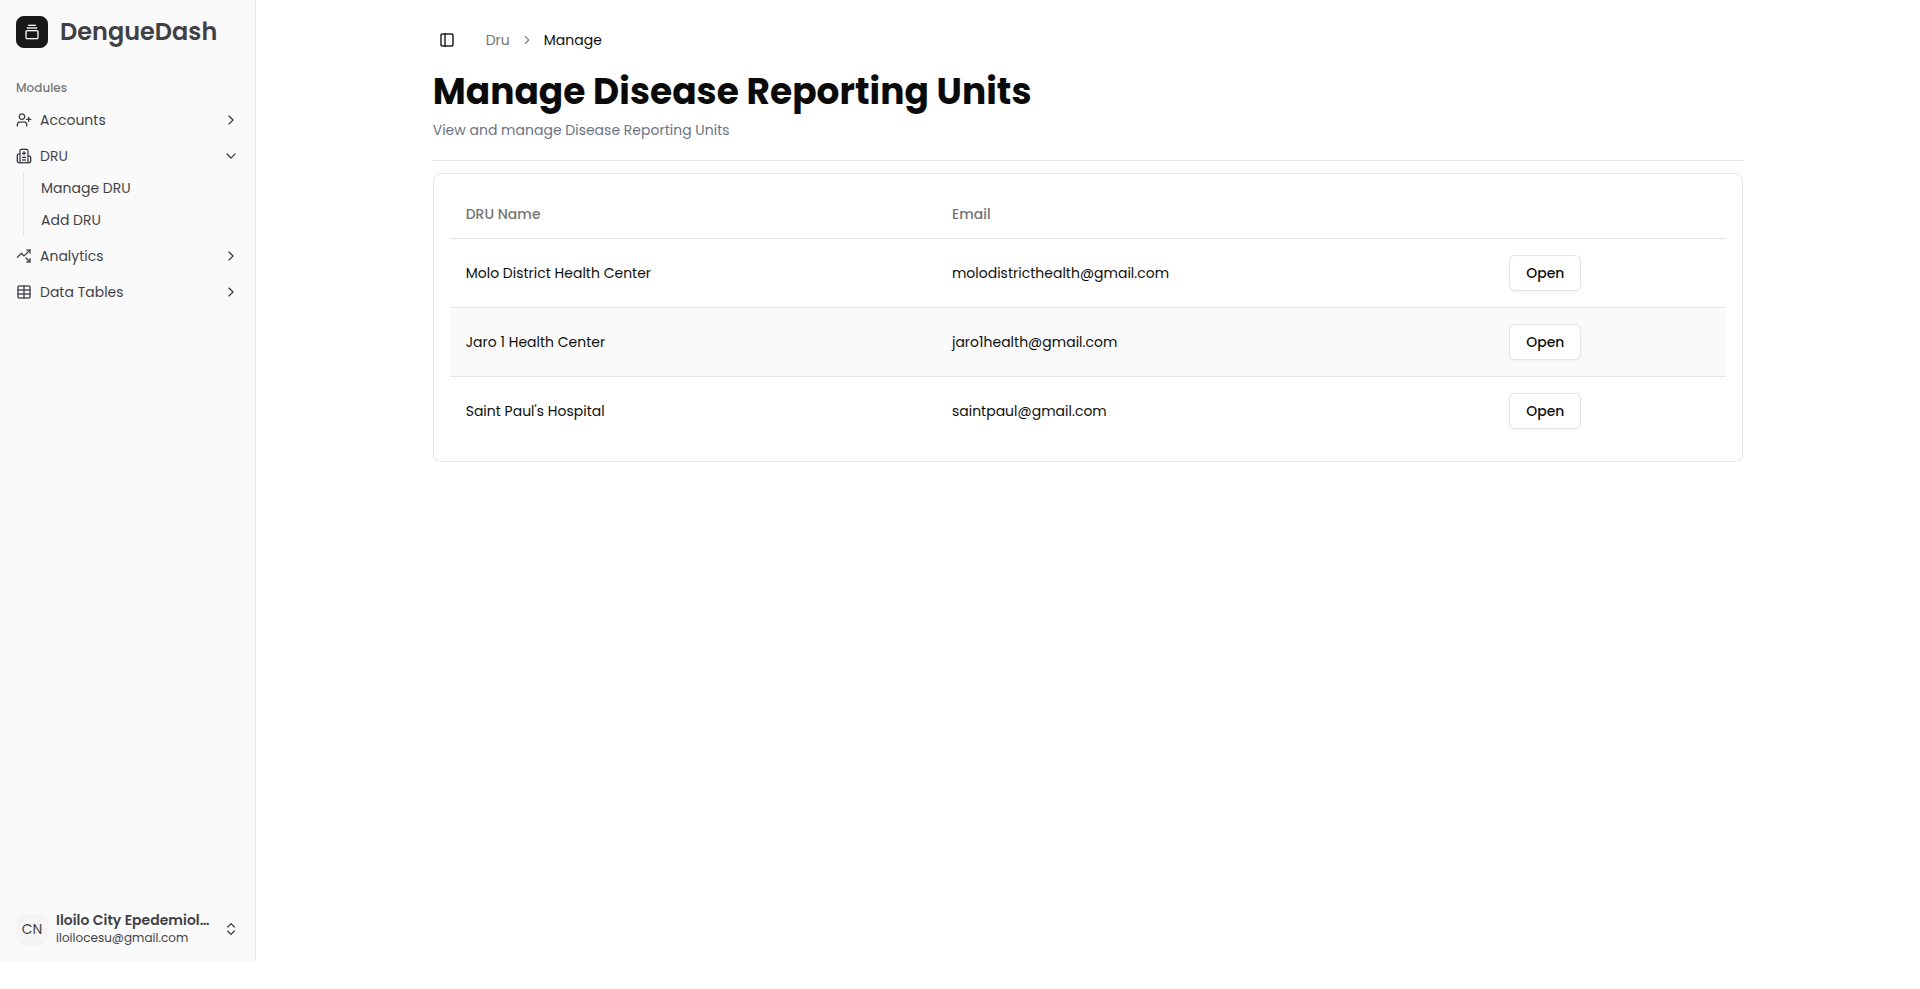
\includegraphics[width=1\textwidth]{browse_drus}
	\caption{List of DRUs}
	\label{fig:browse_drus}
\end{figure}
\begin{figure}[H]
	\centering
	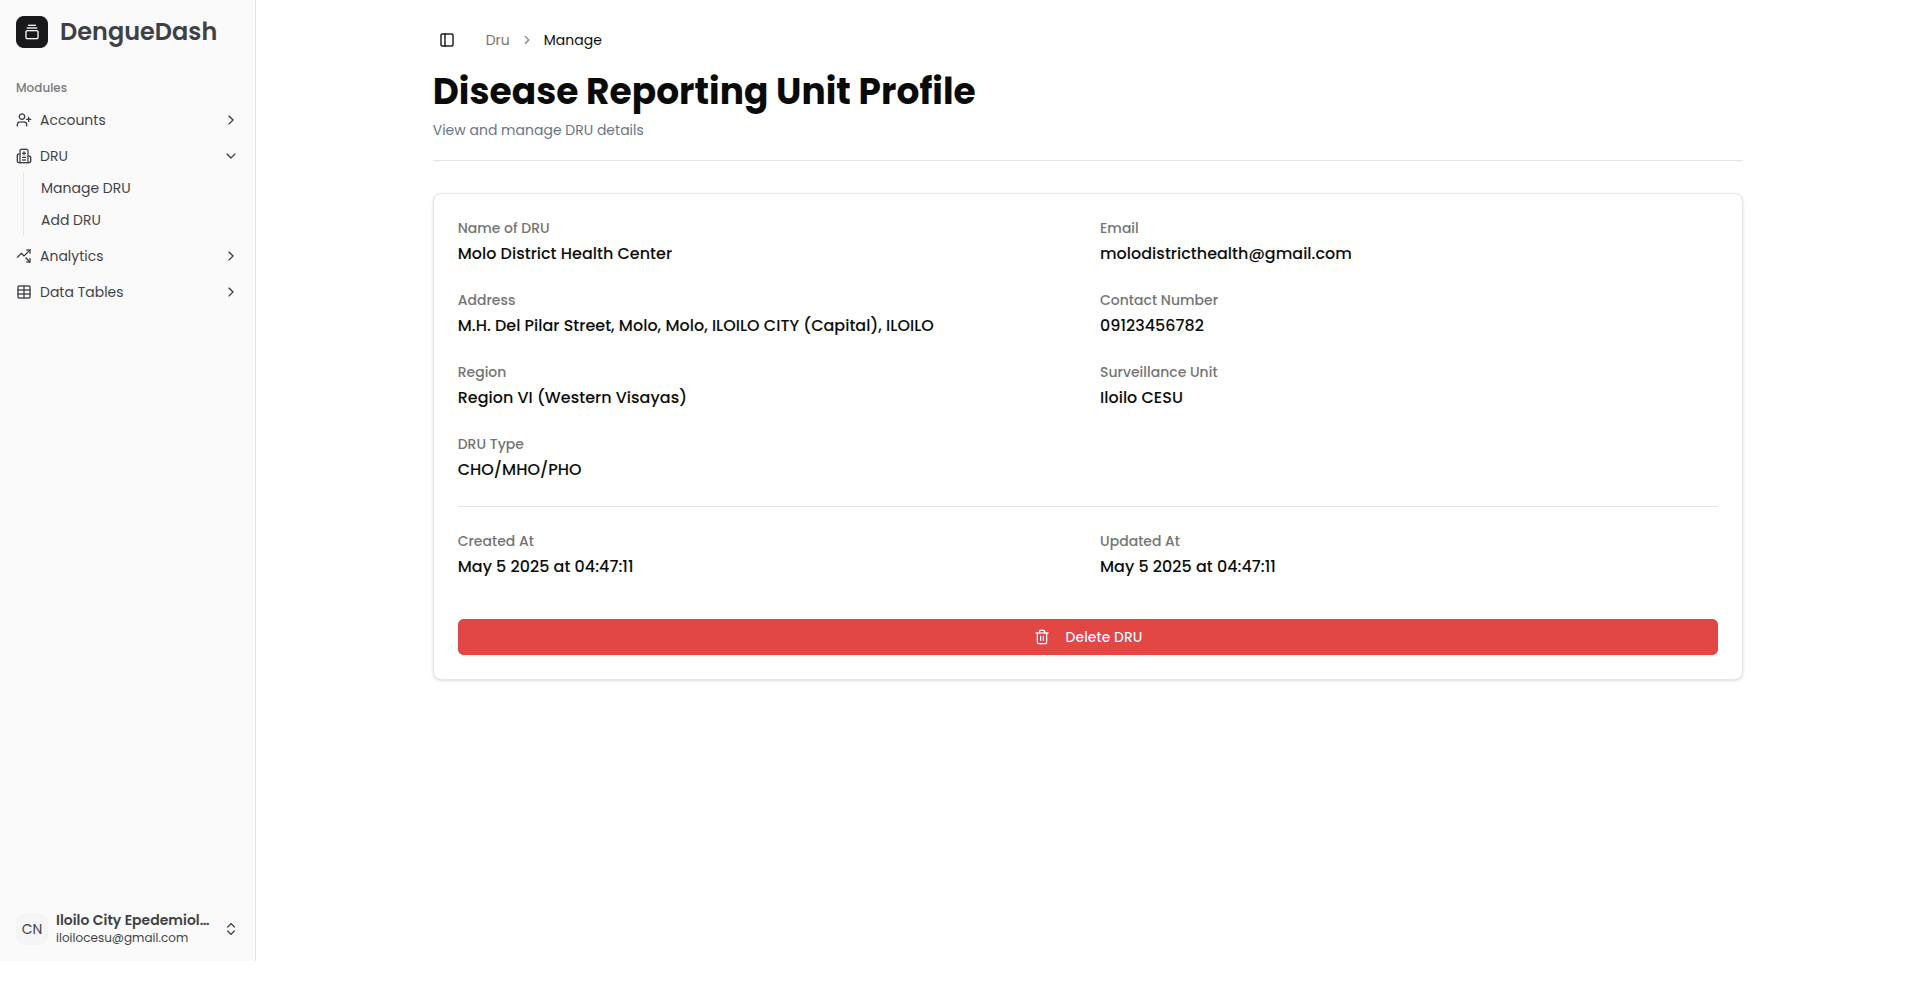
\includegraphics[width=1\textwidth]{dru_details}
	\caption{DRU details}
	\label{fig:dru_details}
\end{figure}


\section{User Testing}
To evaluate the usability of the system, the System Usability Scale (SUS) was utilized. SUS is a Likert-scale-based questionnaire comprising 10 items that are critical to assessing system usability. A total of five participants completed the survey. Their responses were processed following the step-by-step calculation method adopted from \cite{babich_sus_usability_website}. The resulting usability scores for each participant are shown in Table~\ref{tab:sus_scores}.

\begin{table}[h!]
	\centering
	\begin{tabular}{|c|c|}
		\hline
		\textbf{Participant} & \textbf{Usability Score} \\
		\hline
		1 & 95.0 \\
		2 & 90.0 \\
		3 & 85.0 \\
		4 & 87.5 \\
		5 & 85.0 \\
		\hline
		\textbf{Average} & \textbf{88.5} \\
		\hline
	\end{tabular}
	\caption{Computed System Usability Scores per Participant}
	\label{tab:sus_scores}
\end{table}

The average System Usability Scale (SUS) score across systems is typically 68~\cite{babich_sus_usability_website}. In this testing, the system achieved an average SUS score of 88.5, indicating a highly positive user experience. This score suggests that participants found the system not only enjoyable to use but also intuitive enough to recommend to others. Furthermore, it demonstrates that the system is suitable for real-world applications without presenting significant complexity for first-time users.



\section{Conclusion}
\textbf{Revolutionizing Dengue Surveillance: The Rise of AI-Driven Forecasting}

The development of DengueWatch marks a transformative leap forward in public health technology, providing Iloilo City with a centralized system to combat one of the most persistent mosquito-borne diseases. Previously, data was recorded manually on paper, making tracking and analysis slow and error-prone. DengueWatch digitizes this process, enabling faster, more accurate monitoring. More than an academic project, DengueWatch serves as a practical solution aimed at shifting the approach from reactive outbreak response to proactive prevention. By combining deep learning models with real-time climate data integration, the system achieves a level of accuracy and usability that makes it viable for real-world deployment.

At the heart of DengueWatch is a Long Short-Term Memory (LSTM) neural network, which outperformed traditional forecasting models such as ARIMA and Kalman Filter. The LSTM model achieved a Root Mean Square Error (RMSE) of 16.30, compared to 39.00 and 38.40 for ARIMA and Kalman, respectively—demonstrating a substantial improvement in predictive capability. This advantage stems from the LSTM's ability to capture long-term dependencies and model nonlinear relationships between environmental factors and disease patterns.

The analysis also revealed that climate indicators, particularly rainfall and humidity, play a significant role in dengue outbreaks, typically leading to a surge in cases three to five weeks after anomalies are detected. By incorporating these lagged effects, DengueWatch achieved an explanatory power of 83\% (R² = 0.83), offering a game-changing advantage for early intervention and resource allocation.

Usability testing further underscored DengueWatch’s readiness for real-world deployment. The system achieved an average System Usability Scale (SUS) score of 88.5, significantly above the industry benchmark of 68. This indicates that users found the system intuitive, efficient, and suitable for operational use in public health contexts. Key features such as a user-friendly dashboard, a two-week forecasting window aligned with mosquito life cycles, and automated outbreak alerts ensure that the system supports timely, effective responses.

Beyond its immediate application in Iloilo City, the framework behind DengueWatch holds the potential for broader impact. With minor adaptations, it can be scaled nationally through integration with Department of Health surveillance systems.

DengueWatch exemplifies how deep learning can bridge the gap between data science and life-saving interventions. It empowers health workers to act preemptively, policymakers to allocate resources strategically, and communities to engage in early preventive measures. As climate change accelerates the spread of vector-borne diseases, systems like DengueWatch will become indispensable in safeguarding public health. This system not only demonstrates the power of AI in epidemiological forecasting but also lays the foundation for a smarter, more resilient approach to combating infectious diseases in the years ahead.

\textbf{Keywords:} Predictive epidemiology, LSTM neural networks, climate-health modeling, decision support systems, outbreak early warning





